\section{Systematic uncertainties}
\label{sec:strong:syst}

The sources of systematic uncertainty discussed in Sections \ref{sec:common_syst} and \ref{sec:common_backgrounds} are included in the analysis.
The relative size of these uncertainties after the fit in the \glspl{cr} is shown in Figures \ref{fig:syst_cutandcount} and \ref{fig:syst_multibin},
for the cut-and-count and multi-bin analyses respectively. 
In the figure, the uncertainties are grouped into:
\begin{itemize}
\item Experimental uncertainties, which contain the sum in quadrature of the detector-related uncertainties 
presented in Section \ref{sec:common_syst}. These are considered for both the background and signal \gls{mc} samples.
The ranking of the different sources of uncertainty changes from region to region; in general the dominant ones are \gls{jes} (that has a 
relative impact on the expected background between 4 and 35\% in the different \glspl{sr}), \gls{jer} (0-26\%) and the uncertainties on the 
$b$-tagging efficiency and mistagging rate (3--24\%).

\item Theoretical uncertainties, which are the sum in quadrature of the modeling uncertainties discussed in Section \ref{sec:common_backgrounds}.
In this case the dominant uncertainties are the ones on the modeling of the \ttbar background, whose impact ranges between 5 and 76\%.

\item \gls{mc} statistical uncertainty.

\item Statistical uncertainty in the \glspl{cr}, that is reflected in the uncertainty in the \ttbar scale factor and takes values between 10 and 30\%.

\end{itemize}

The total uncertainty (black line in Figure \ref{fig:syst}) takes into account correlation effects across the different systematic sources, 
and therefore is not equal to the sum in quadrature of the individual components. 

\begin{figure}[htbp]
	\centering
	\subfigure[]{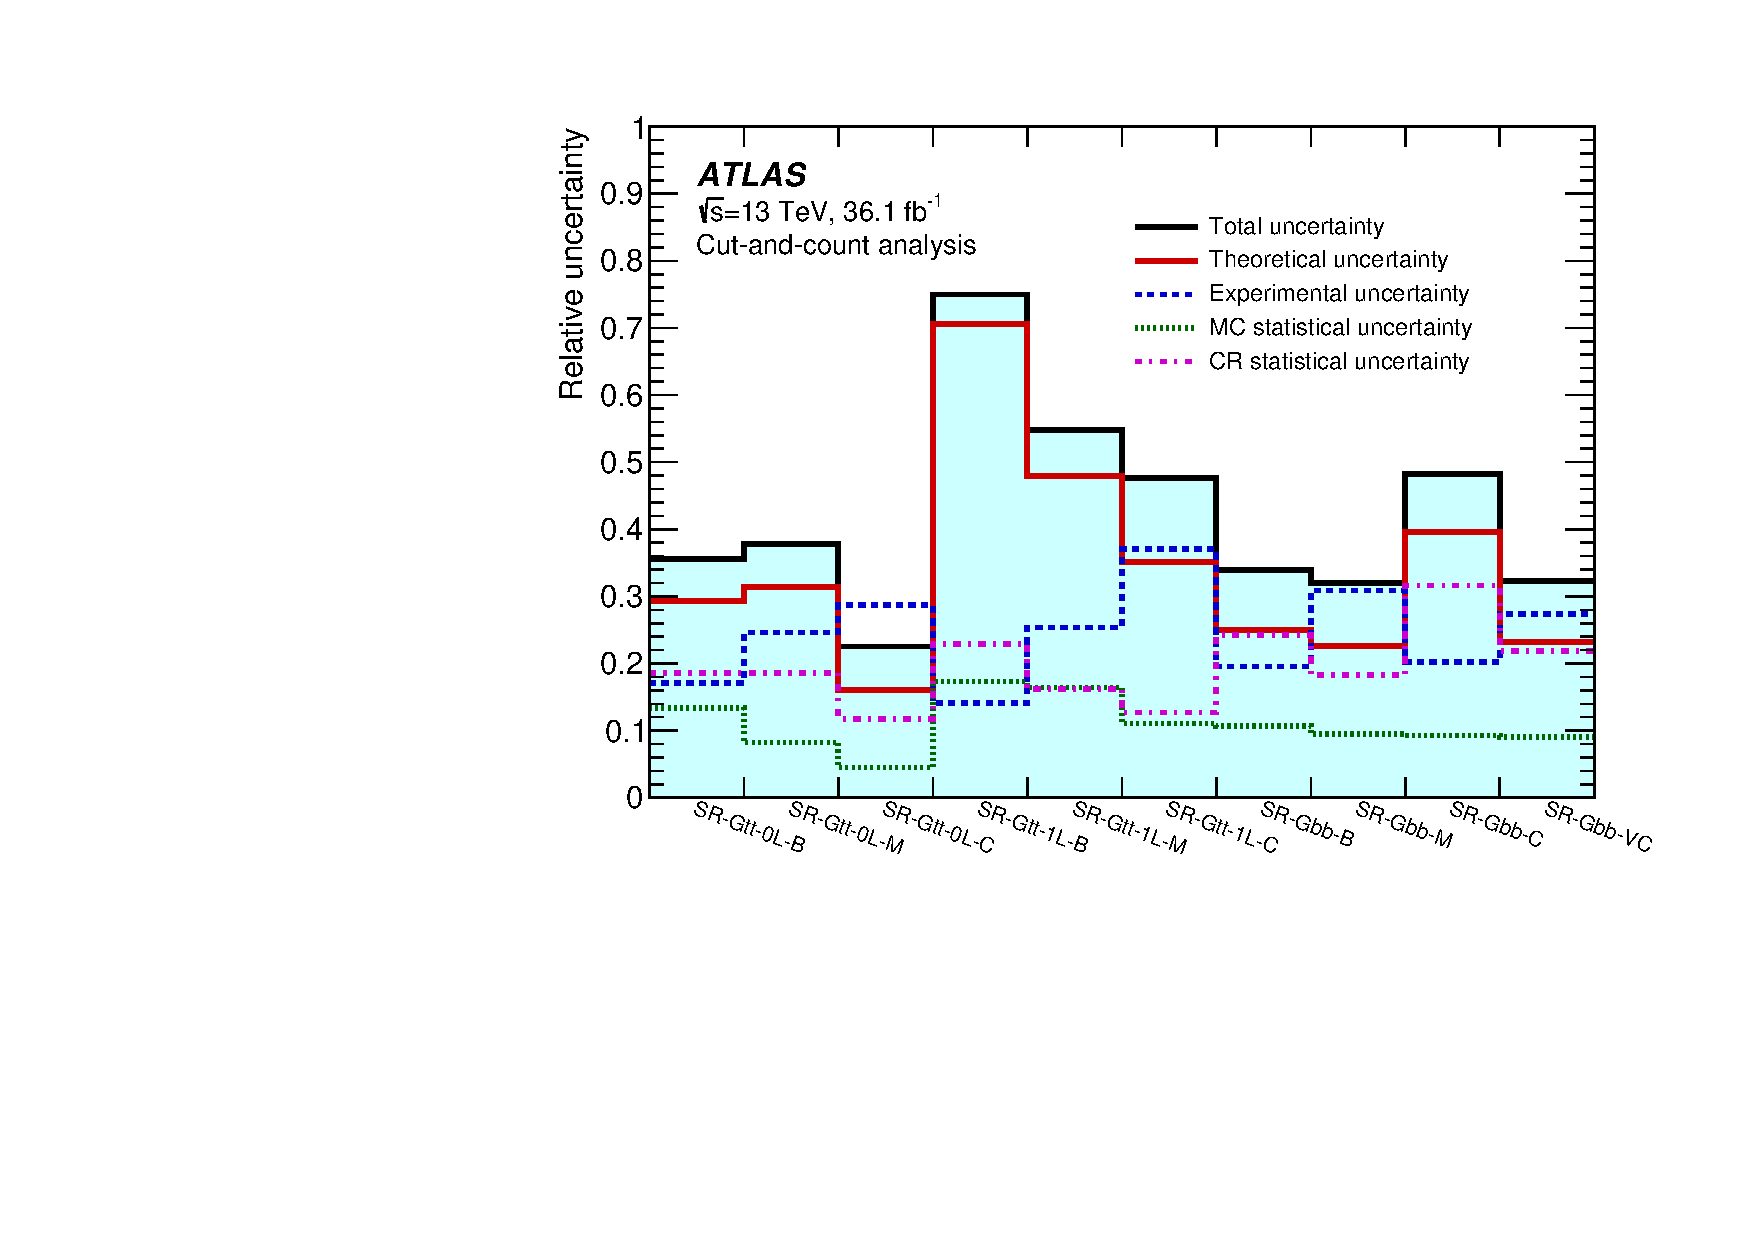
\includegraphics[width=0.85\textwidth]{figures/strong_prod/paper/Cut_and_Count.pdf}\label{fig:syst_cutandcount}}\\
	\subfigure[]{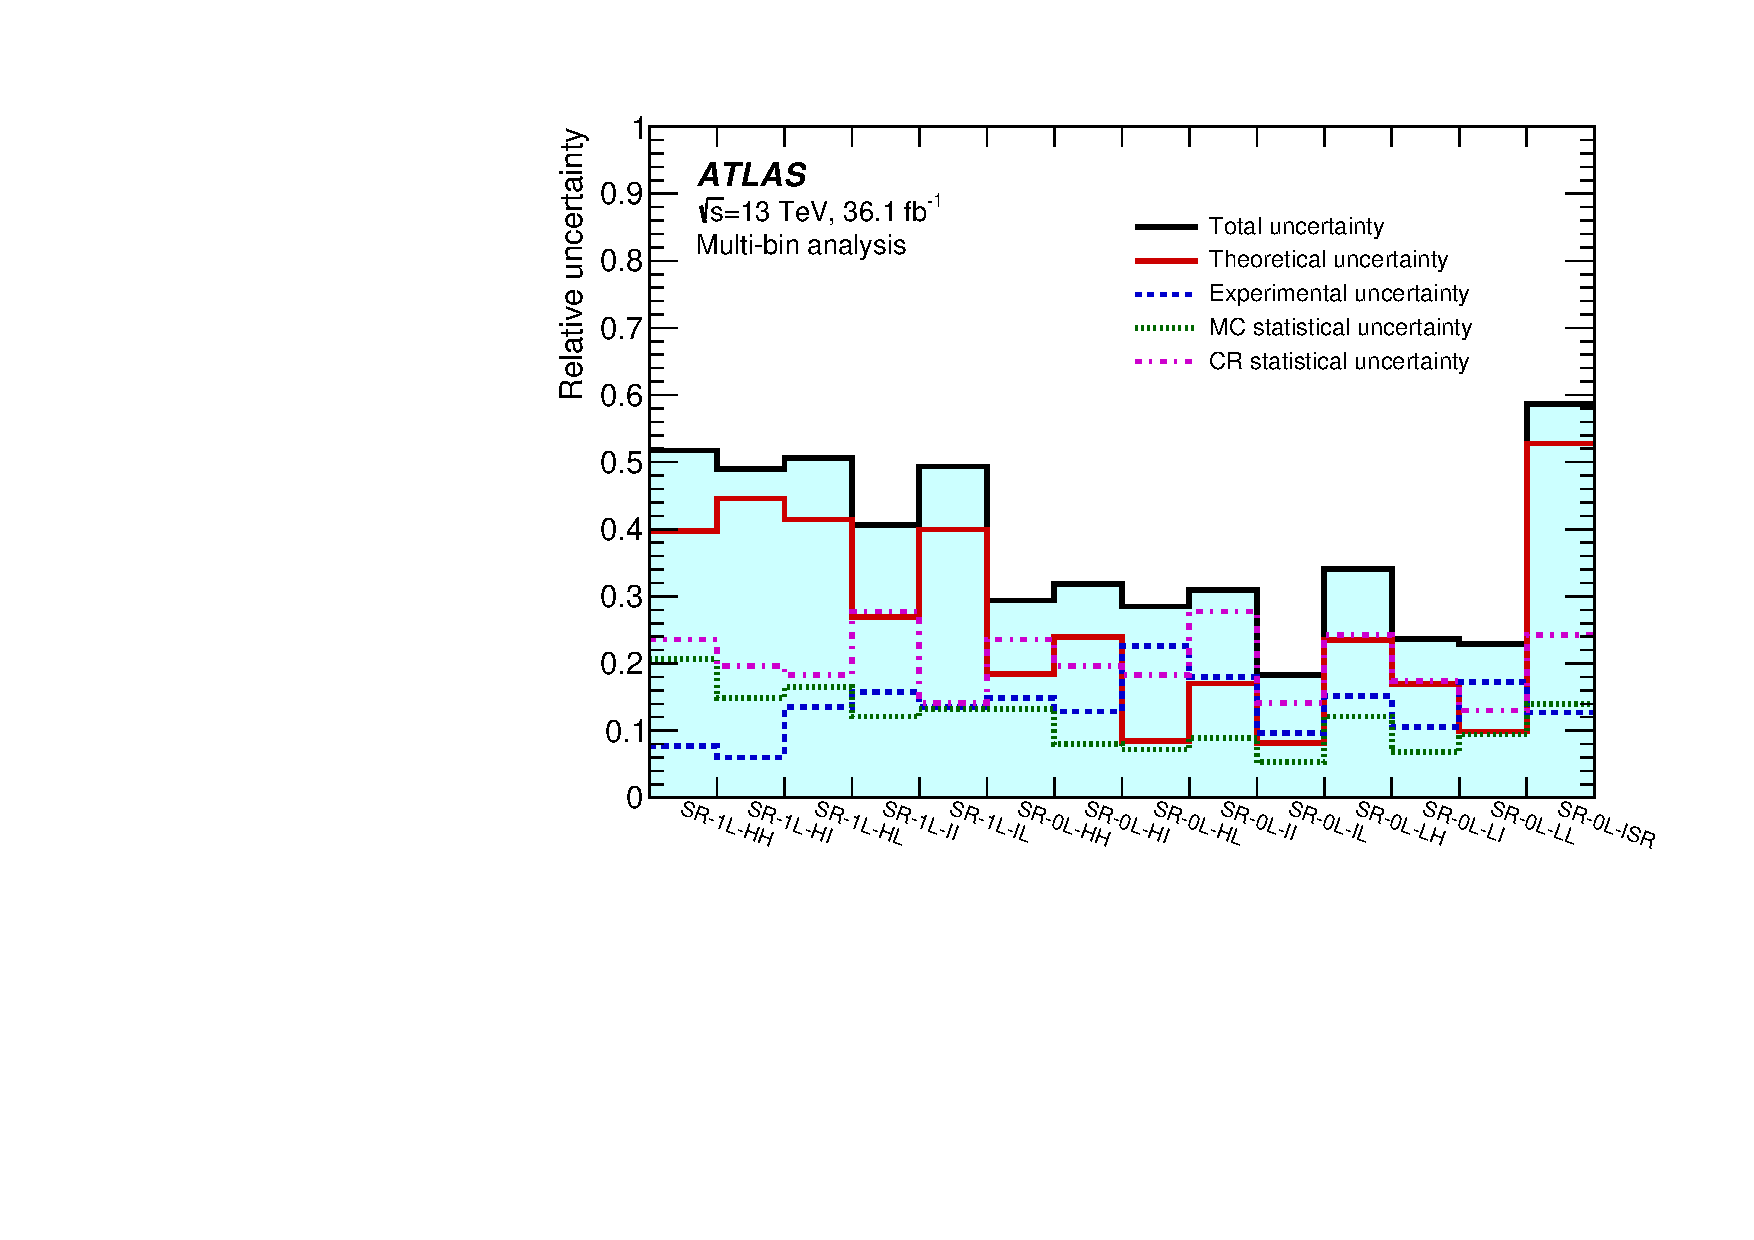
\includegraphics[width=0.85\textwidth]{figures/strong_prod/paper/Multi_bin.pdf}\label{fig:syst_multibin}}\\
	\caption{Relative systematic uncertainty in the background estimate for \subref{fig:syst_cutandcount} the cut-and-count and \subref{fig:syst_multibin} the multi-bin analyses. The individual uncertainties can be correlated, such that the total background uncertainty is not necessarily their sum in quadrature.  Figure from Ref. \cite{Aaboud:2017hrg}.
	} 
	\label{fig:syst}
\end{figure}

\section{Results}
\label{sec:strongprod:results}

The statistical procedures discussed in Chapter \ref{chap:stat} are used to compare the simulations and the data, and to extract 
quantitative information on their agreement and on the presence of \gls{bsm} signals. 
The first step is the background-only fit, a maximum-likelihood fit where only the \glspl{cr} are included, as described in Section 
\ref{sec:example_cr}. 
The \ttbar normalization is a free parameter of the fit, and is therefore adjusted with the number of observed events in the \glspl{cr} 
as constraint.
This procedure accounts for potential mismodelings specific of the kinematic regime close to each \gls{sr}, which are not necessarily 
the same for all the regions in the analysis. Therefore each \gls{cr} is used to derive a normalization factor for the \ttbar background,
independent from the normalization factors derived in the other \glspl{cr}, that is then used to derive the background prediction in the 
corresponding \glspl{sr}. 

The top panel of Figures \ref{fig:pullCR_discovery} and \ref{fig:pullCR_exclusion} shows the 
comparison between data and simulation in the 
\glspl{cr} of the cut-and-count and multi-bin analyses respectively. In the same figures, the bottom panel 
shows the \ttbar normalization factor derived from the fit in the \glspl{cr} with the associated uncertainty, driven by the statistical uncertainty 
in the \glspl{cr}.  The systematic uncertainties on the expected number of events are included in the fit as nuisance parameters.
Note that in the case of the cut-and-count analysis the fit is performed separately in each \gls{cr}, 
while for the multi-bin analysis all the \glspl{cr} are included in the same fit, even though with independent parameters for the 
\ttbar normalization. 
 

\begin{figure}[htbp]
	\centering
	\subfigure[]{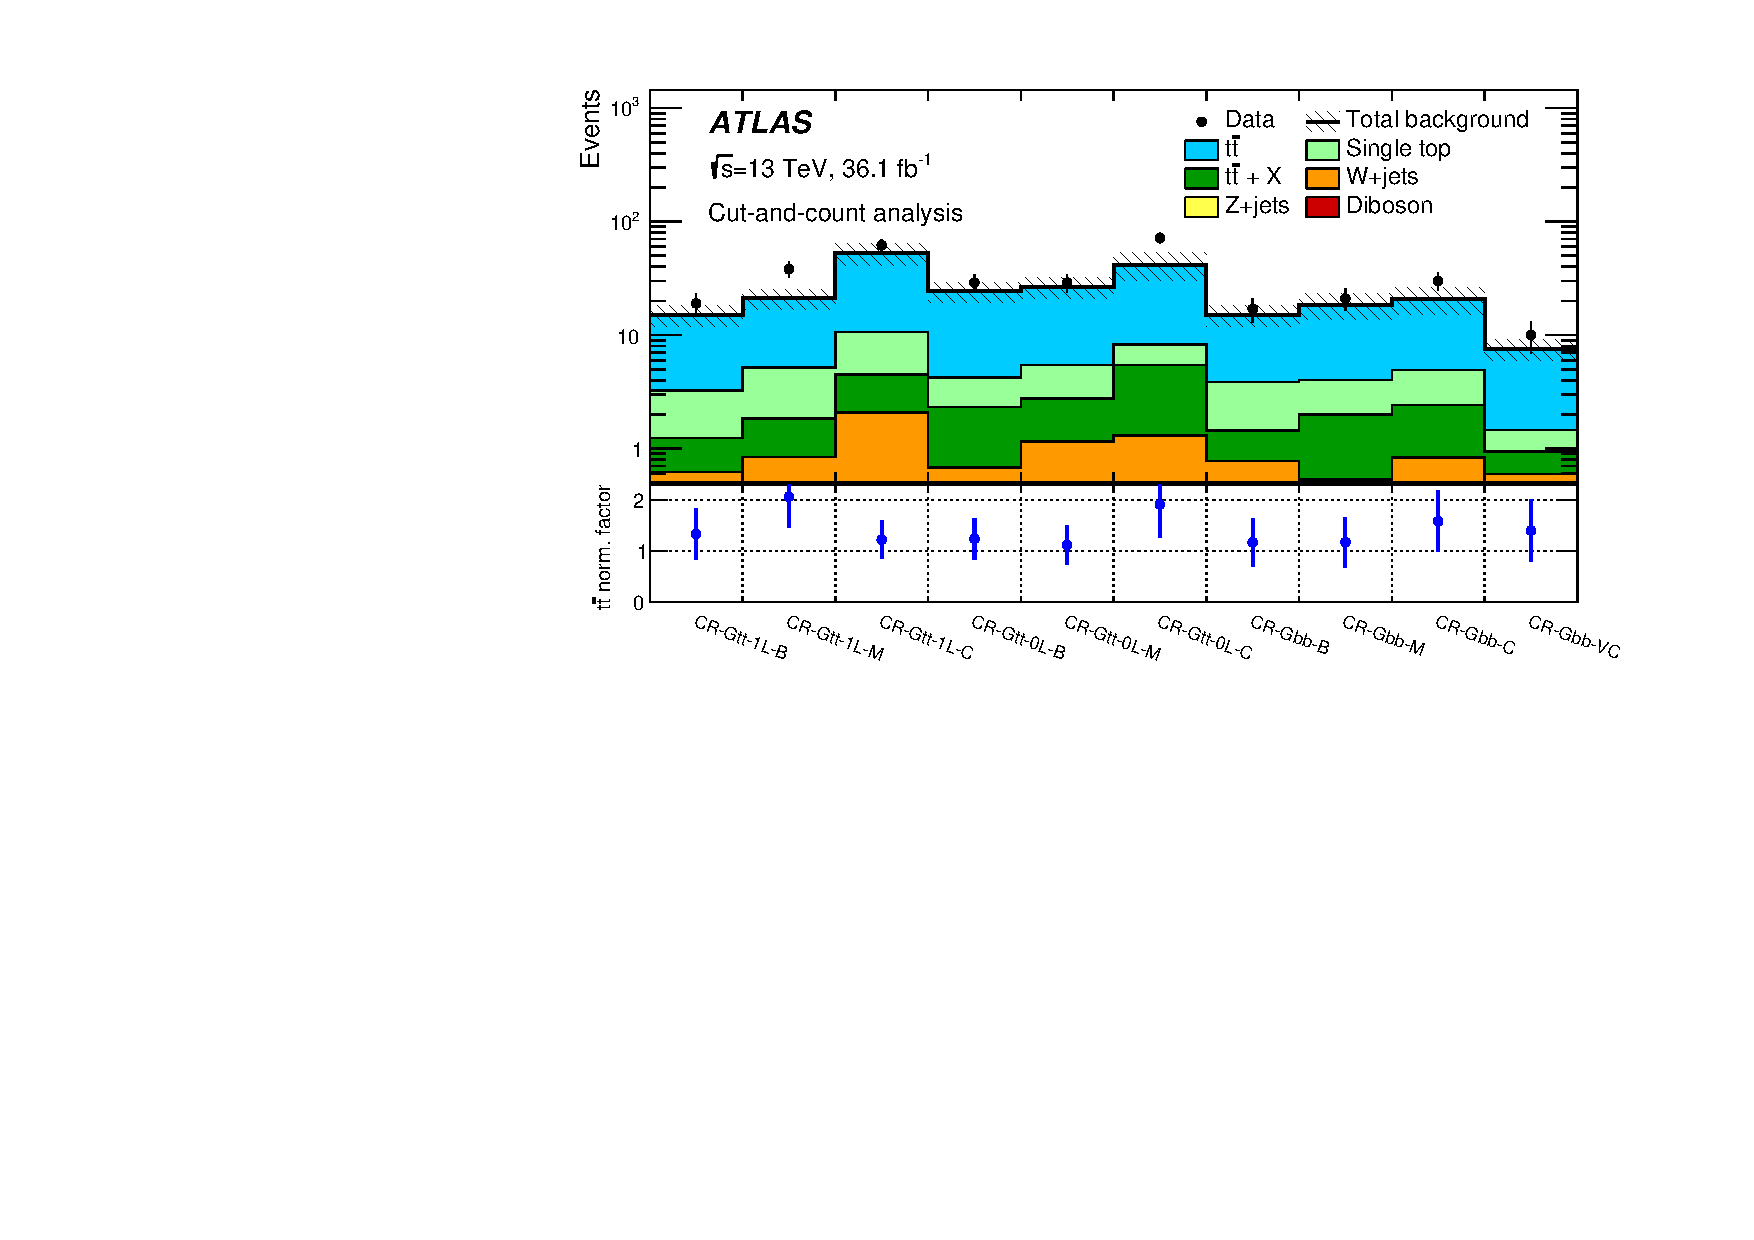
\includegraphics[width=0.9\textwidth]{figures/strong_prod/paper/pulls/histpull_pulls_in_CRs_17_06_23_singlebin.pdf}\label{fig:pullCR_discovery}}
	\subfigure[]{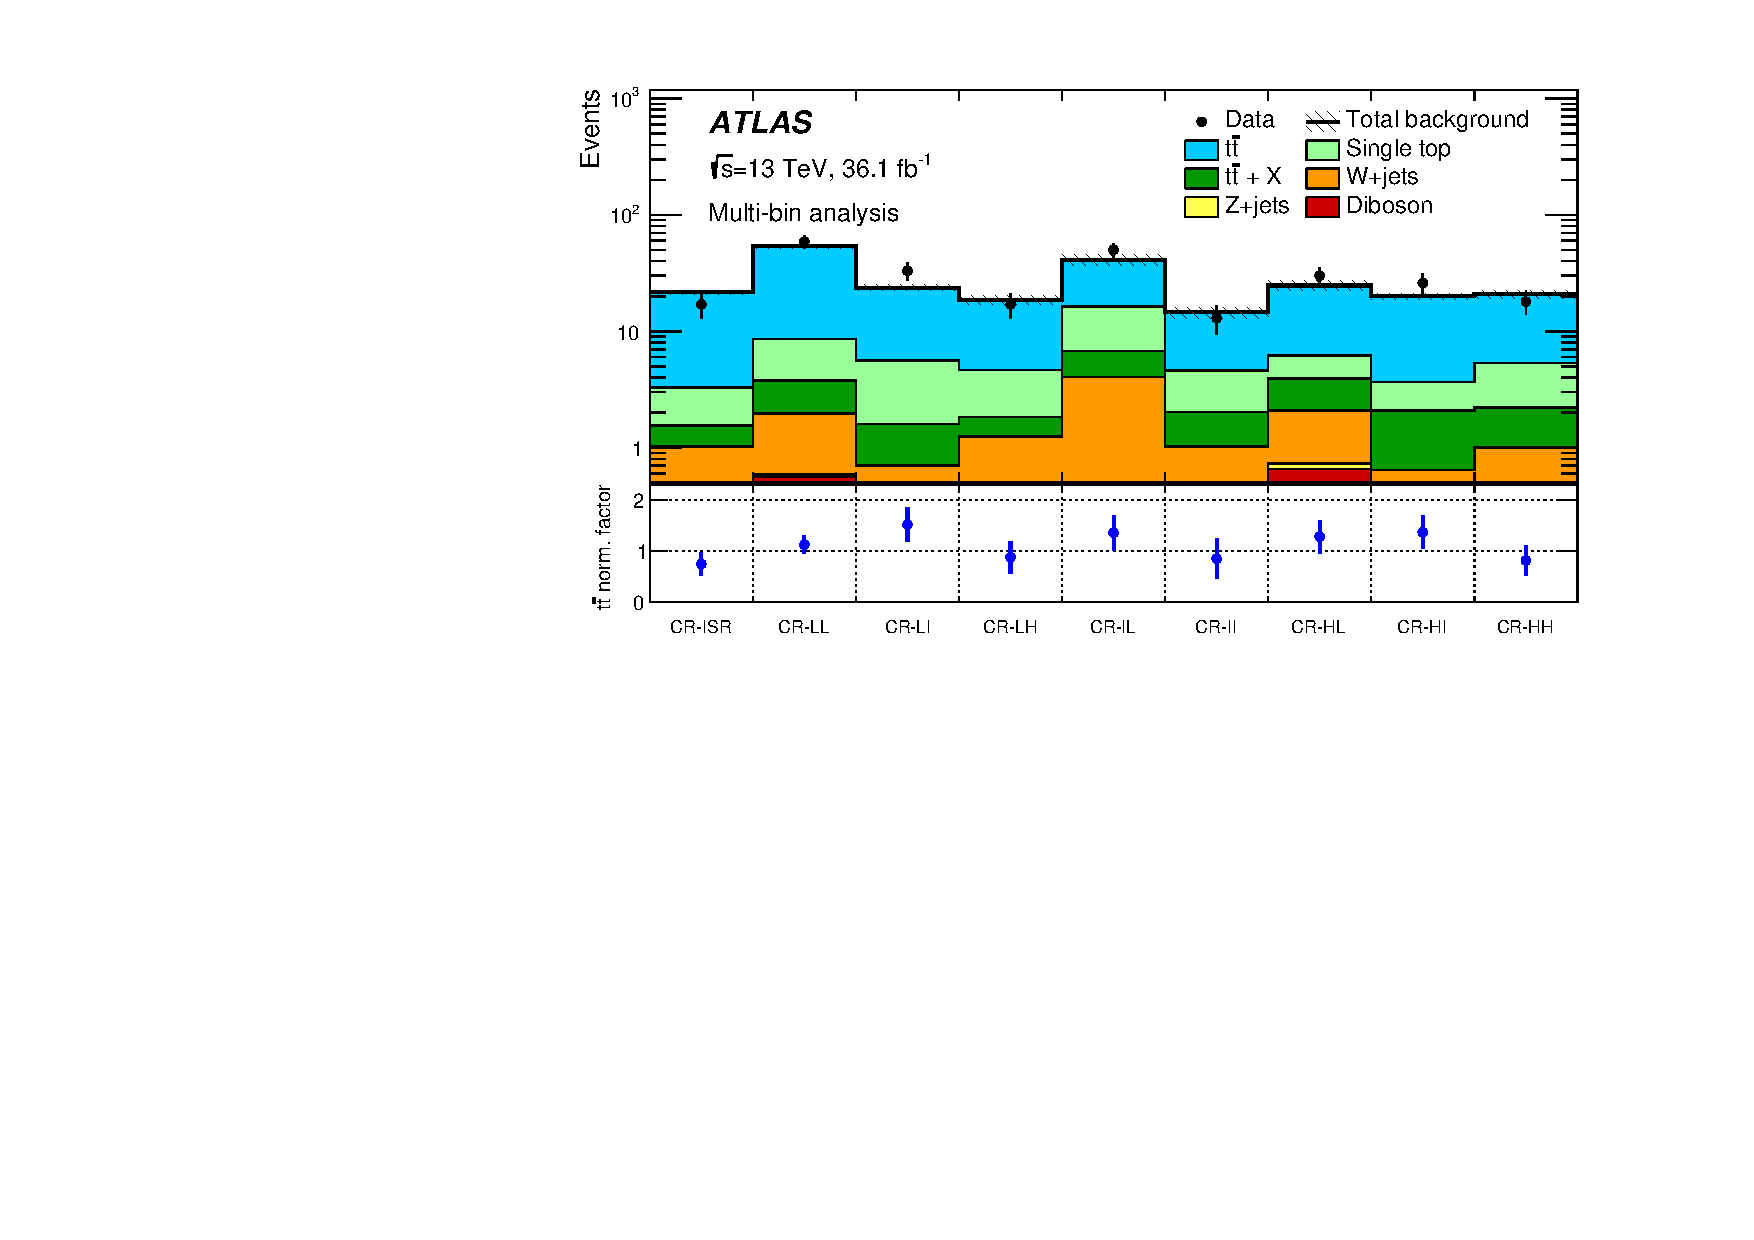
\includegraphics[width=0.9\textwidth]{figures/strong_prod/paper/pulls/histpull_pulls_in_CRs_multichannel_17_06_23.pdf}\label{fig:pullCR_exclusion}}
	\caption{Pre-fit event yield in \glspl{cr} and related \ttbar
          normalization factors after the background-only fit for
          \subref{fig:pullCR_discovery} 
		the cut-and-count and \subref{fig:pullCR_exclusion} the multi-bin analyses. The upper panel shows 
		the observed number of events and the predicted background yield before the fit.
		The background category \ttbar+X includes \ttbar+W/Z, \ttbar+H and \ttbar\ttbar events. All of these
                regions require at least one signal lepton, for which the
                multijet background is negligible. All uncertainties described in Section \ref{sec:strong:syst} are included in the uncertainty band.
		The \ttbar normalization is obtained from the fit
                and is displayed in the bottom panel.  Figures from Ref. \cite{Aaboud:2017hrg}.
	} 
	\label{fig:pullCR}
\end{figure}

Figures \ref{fig:pullVR_discovery} and \ref{fig:pullVR_exclusion} show the result of the background-only fit extrapolated to the \glspl{vr} of 
the cut-and-count and multi-bin analyses respectively. The upper panel shows the comparison of the number of predicted and observed events, 
while the bottom panel quantifies the difference between the expected and the observed with the pull, defined as the difference between 
number of observed and expected events divided by the total uncertainty. 

\begin{figure}[htbp]
	\centering
	\subfigure[]{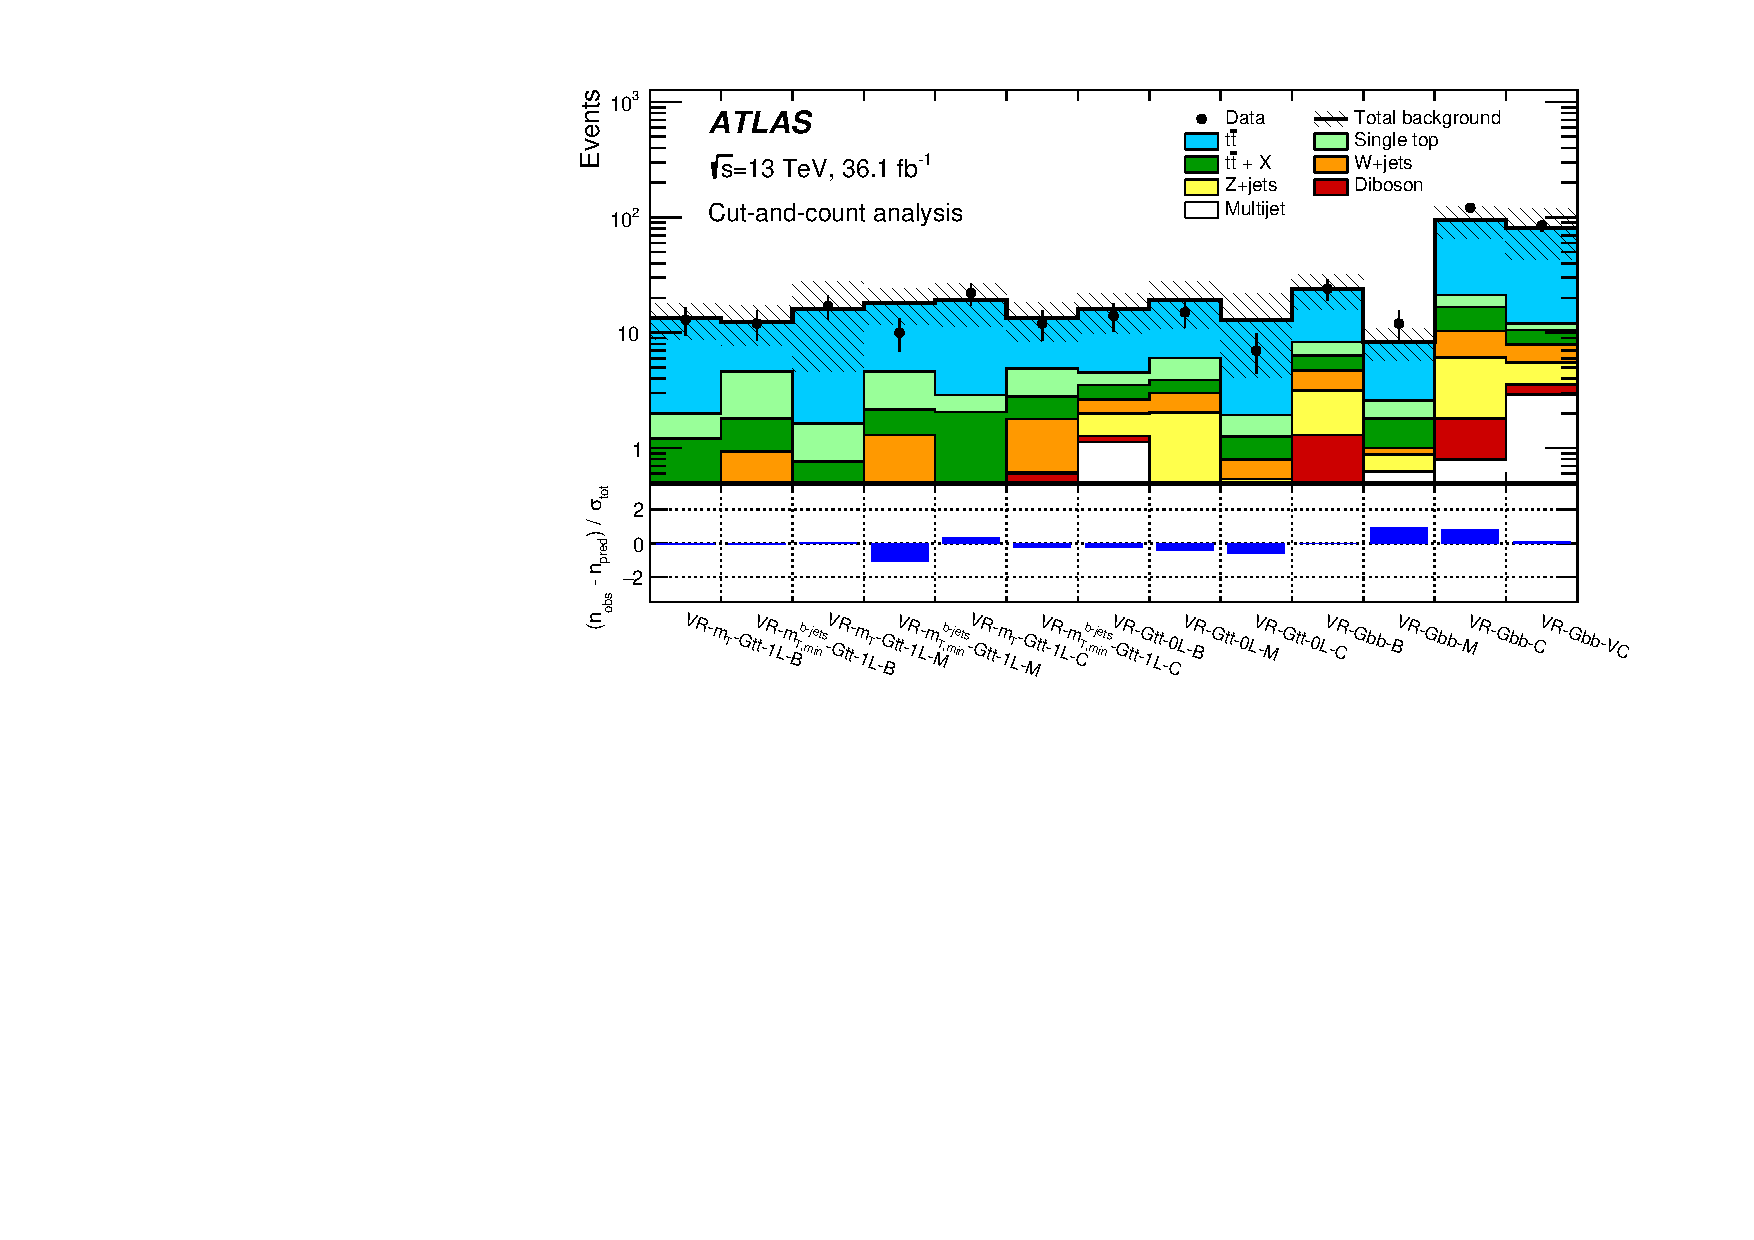
\includegraphics[width=0.9\textwidth]{figures/strong_prod/paper/pulls/histpull_pulls_in_VRs_17_06_23_singlebin.pdf}\label{fig:pullVR_discovery}}\\
	\subfigure[]{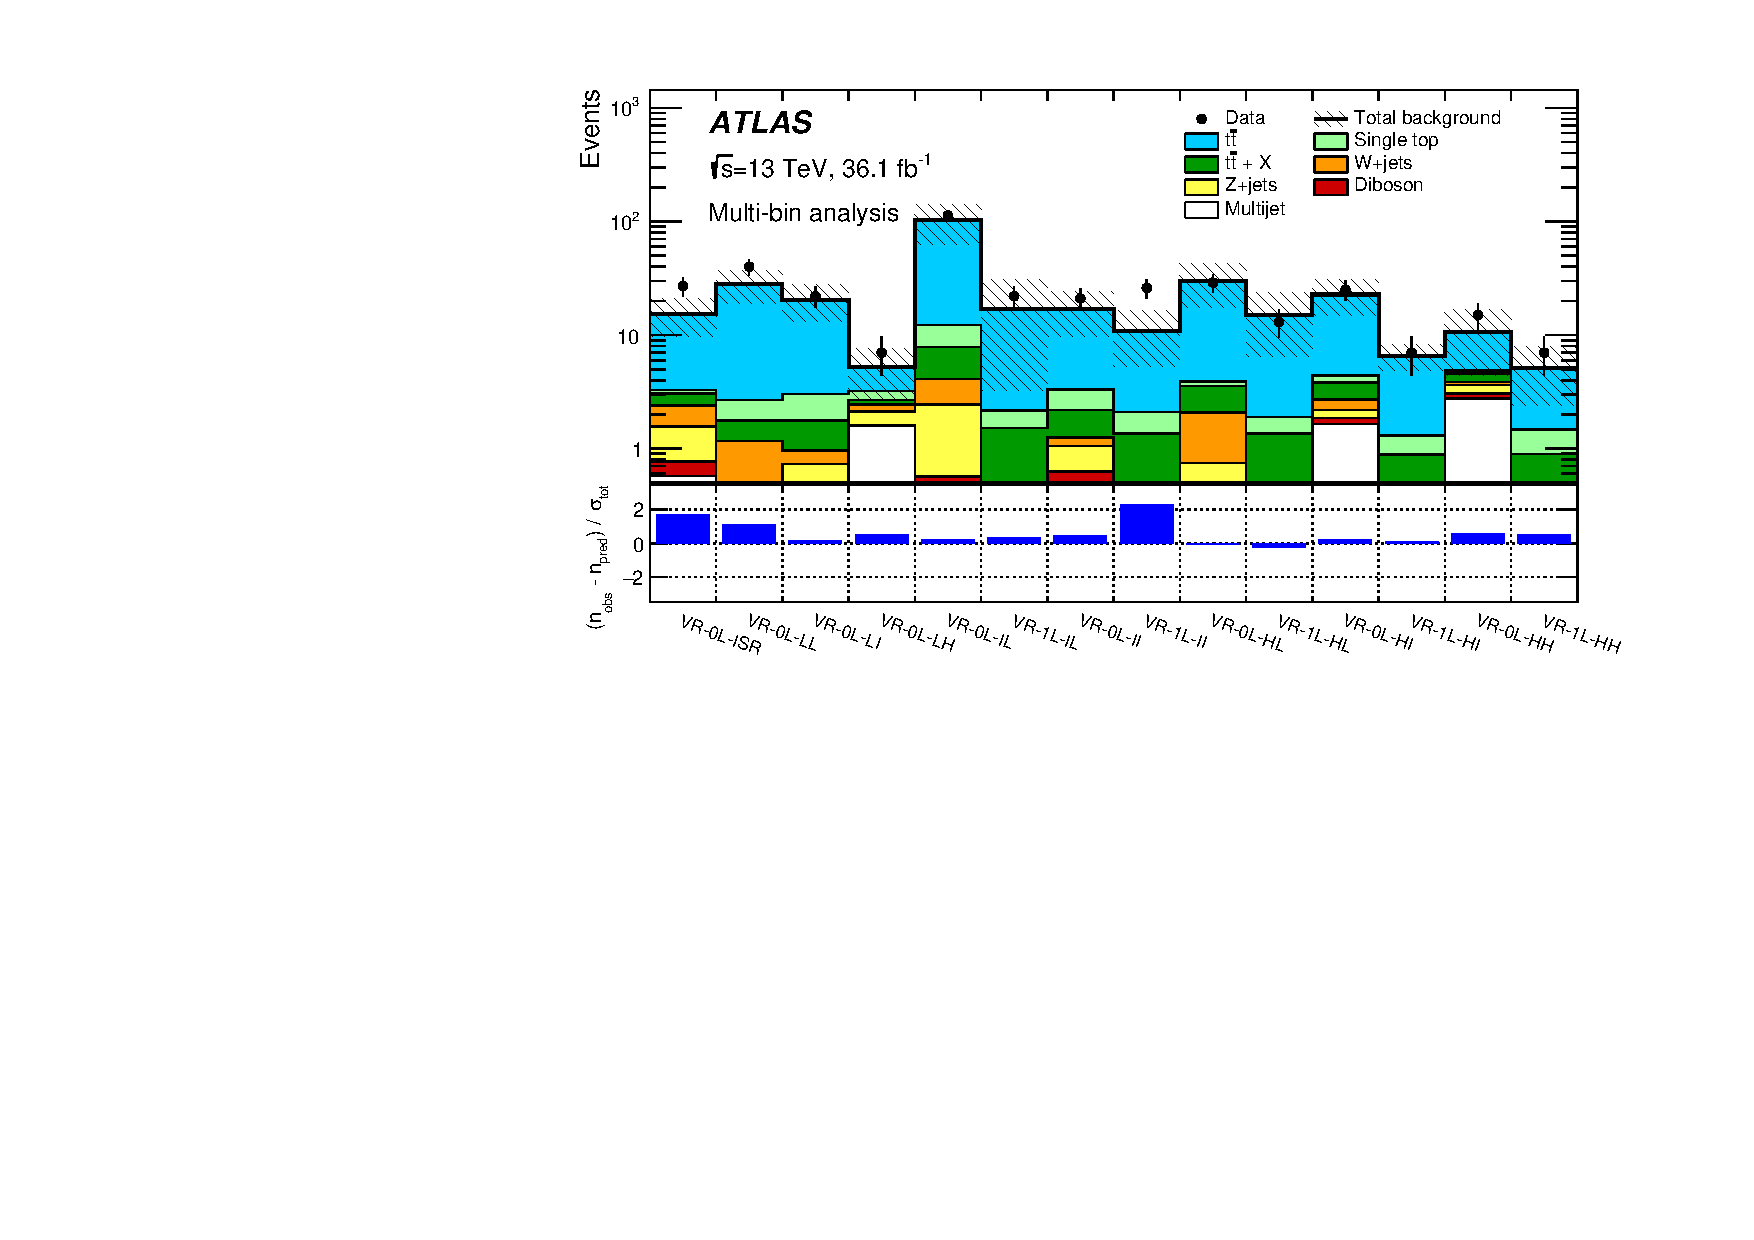
\includegraphics[width=0.9\textwidth]{figures/strong_prod/paper/pulls/histpull_pulls_in_VRs_multichannel_17_06_23.pdf}\label{fig:pullVR_exclusion}}\\
	\caption{Results of the background-only fit extrapolated to the VRs of \subref{fig:pullVR_discovery} the cut-and-count and \subref{fig:pullVR_exclusion}
		the multi-bin analyses. The \ttbar normalization 
		is obtained from the fit to the CRs shown in Figure~\ref{fig:pullCR}. The upper panel shows 
		the observed number of events and the predicted background yield.
		All uncertainties  described in Section \ref{sec:strong:syst} are included in the 
		uncertainty band. The background category \ttbar+X includes \ttbar+W/Z, 
		\ttbar+H and \ttbar\ttbar events. The lower panel shows the pulls in 
		each VR.  Figures from Ref. \cite{Aaboud:2017hrg}.
	} 
	\label{fig:pullVR}
\end{figure}

The result of the fit extrapolated to the \glspl{sr} and the observed number of events in the \glspl{sr} are finally
shown in Figures \ref{fig:pullSR_discovery} and \ref{fig:pullSR_exclusion} 
for the cut-and-count and the multi-bin analyses respectively. 
No significant excess is observed in the \glspl{sr}; the largest excess is observed in SR-0L-HH, 
one of the regions of the multi-bin analysis, where the pull is 2.3 standard deviations. 
The numerical results in the cut-and-count \glspl{sr} are summarized in Table \ref{tab:yield_discovery}.

\begin{figure}[htbp]
	\centering
	\subfigure[]{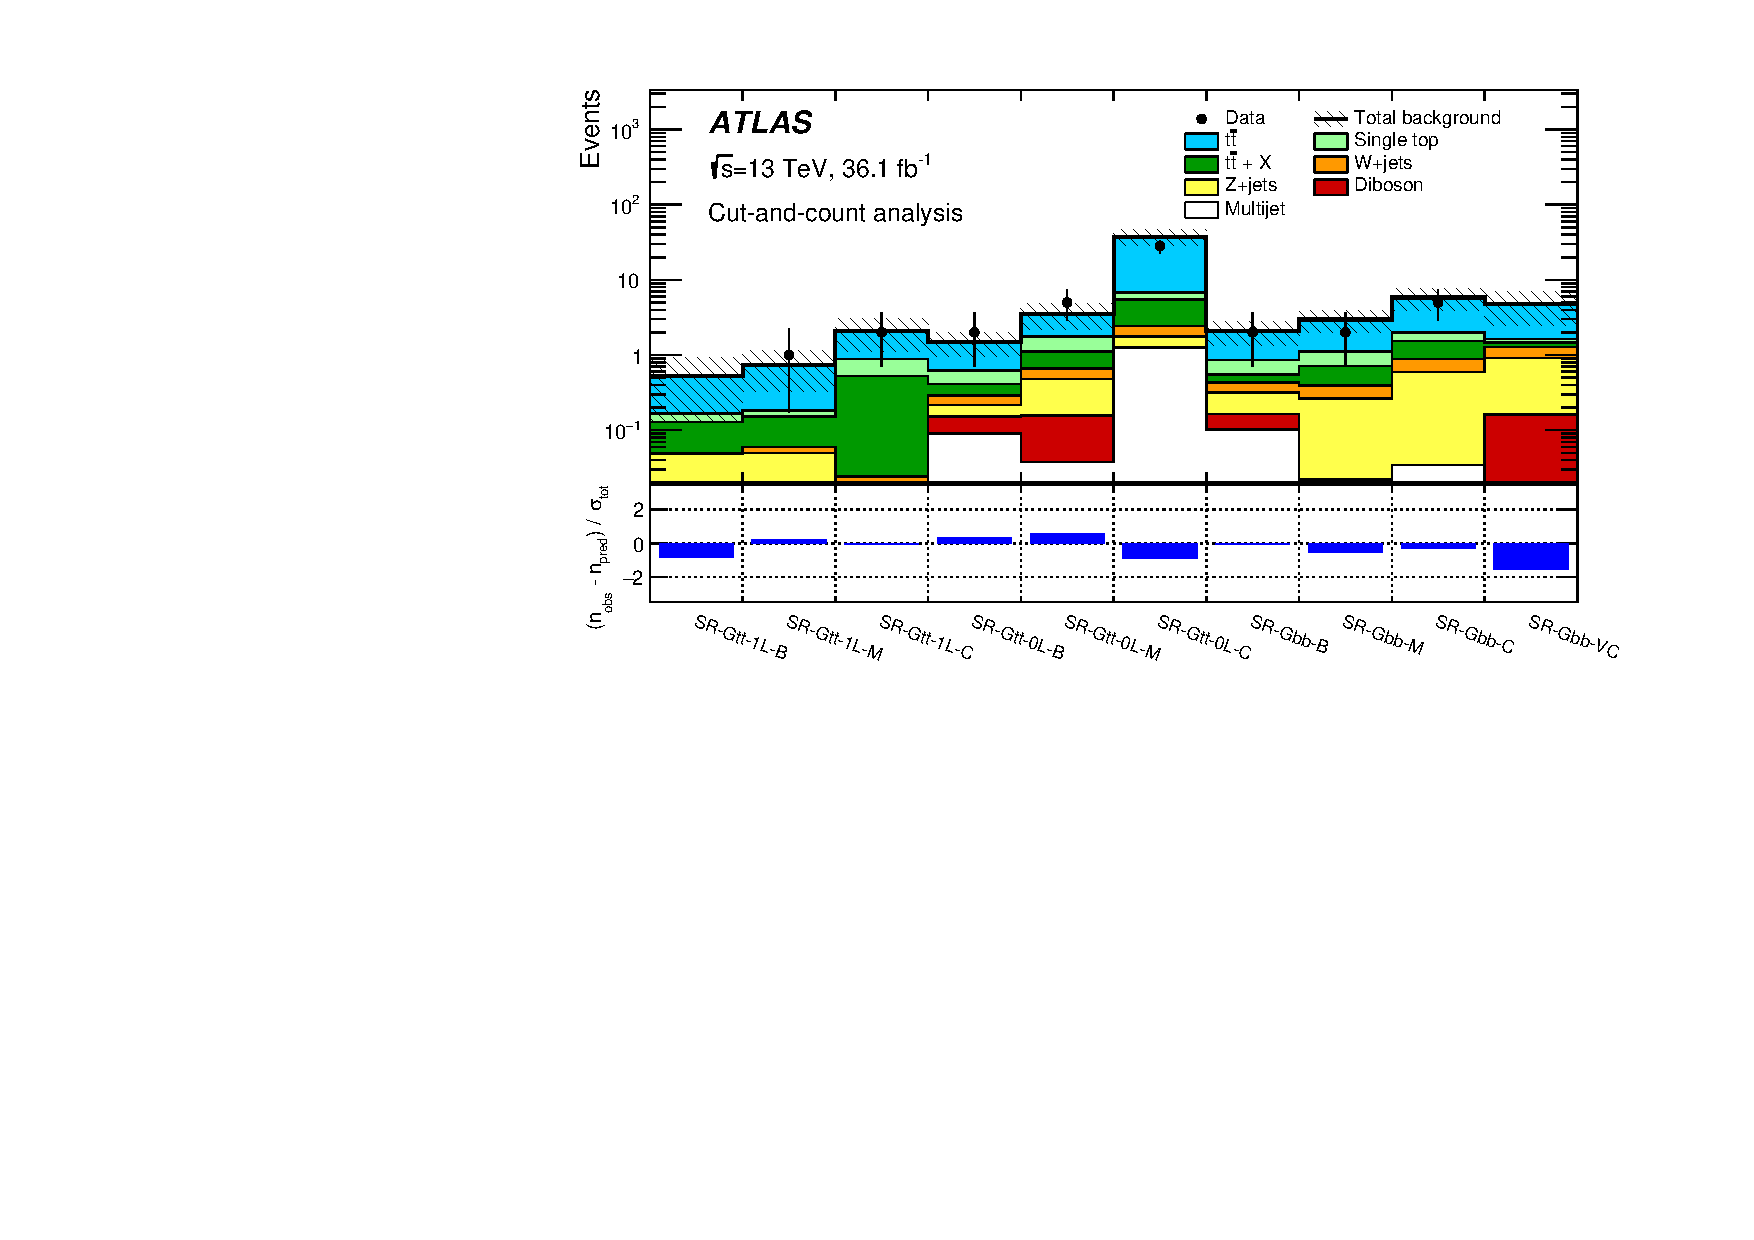
\includegraphics[width=0.9\textwidth]{figures/strong_prod/paper/pulls/histpull_pulls_in_SRs_17_06_23_singlebin.pdf}\label{fig:pullSR_discovery}}\\
	\subfigure[]{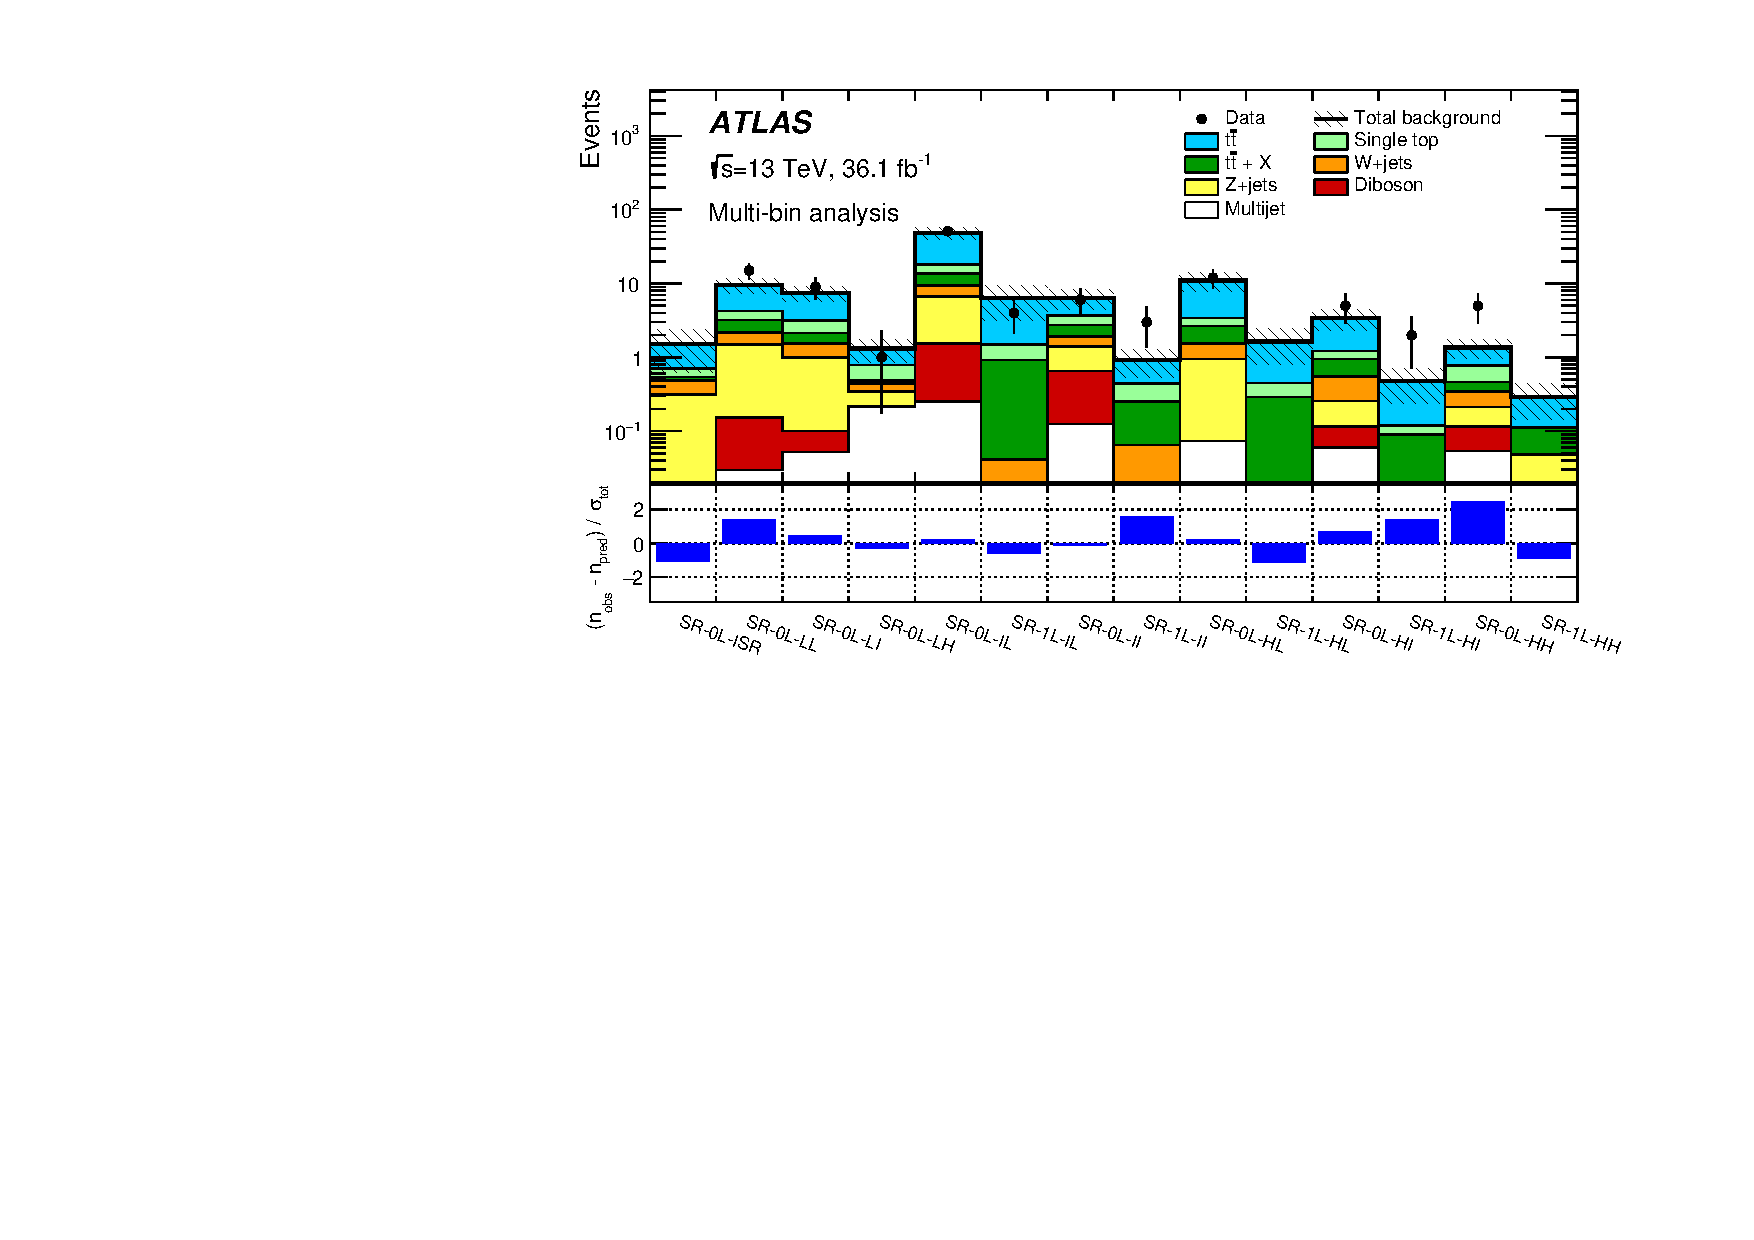
\includegraphics[width=0.9\textwidth]{figures/strong_prod/paper/pulls/histpull_pulls_in_SRs_multichannel_17_06_23.pdf}\label{fig:pullSR_exclusion}}\\
	\caption{Results of the background-only fit extrapolated to the SRs for \subref{fig:pullSR_discovery}
	the cut-and-count and \subref{fig:pullSR_exclusion} the multi-bin analyses. The data in the  SRs are 
	not included in the fit.  The upper panel shows the observed number of events and the predicted background 
	yield. All uncertainties  described in Section \ref{sec:strong:syst} are included in the uncertainty band. The background 
	category $\ttbar+X$ includes $\ttbar W/Z$, $\ttbar H$ and $\ttbar \ttbar$ events. The lower panel shows the 
	pulls in each SR.  Figures from Ref. \cite{Aaboud:2017hrg}.} 
	\label{fig:pullSR}
\end{figure}

\begin{table*}[htbp]
	\centering	
	\renewcommand{\arraystretch}{1.0}
	\begin{tabular}{lccc}
	       \toprule
	       & \multicolumn{3}{c}{SR-Gtt-1L} \\
	       \midrule	
	        Targeted kinematics & B            &   M         &   C               \\[-0.05cm]
	       \midrule
	       Observed events              &  0   &  1 & 2  \\
	       \midrule
	       Fitted background             & 0.5 $\pm$ 0.4 & 0.7 $\pm$ 0.4 & 2.1 $\pm$ 1.0\\
	       \midrule
	       \ttbar\              &  0.4 $\pm$ 0.4 & 0.5 $\pm$ 0.4 & 1.2 $\pm$ 0.8\\
	       Single-top             & 0.04 $\pm$ 0.05 & 0.03 $\pm$ 0.06 & 0.35 $\pm$ 0.28\\
	       $\ttbar+X$          & 0.08 $\pm$ 0.05 & 0.09 $\pm$ 0.06 & 0.50 $\pm$ 0.28\\
	       $Z$+jets            & 0.049 $\pm$ 0.023 & 0.050 $\pm$ 0.023 & $<0.01$ \\
	       $W$+jets              & $<0.01$  & $<0.01$  & 0.024 $\pm$ 0.026\\
	       Diboson             & $<0.01$ & $<0.01$  & $<0.01$ \\
 	       \midrule
	       MC-only background &  0.43 & 0.45 & 1.9 \\
	       \bottomrule
	\end{tabular}

	\vspace{0.4cm}
	
        \begin{tabular}{lccc}
		\toprule
		& \multicolumn{3}{c}{SR-Gtt-0L} \\
		\midrule	
	       Targeted kinematics & B            &   M         &   C               \\[-0.05cm]
	       \midrule
	       Observed events              &  2 & 5 & 28 \\
	       \midrule
	       Fitted background             & 1.5 $\pm$ 0.5 & 3.5 $\pm$ 1.3 & 38 $\pm$ 8\phantom{0} \\
	       \midrule
	       \ttbar\              & 0.9 $\pm$ 0.4 & 1.8 $\pm$ 0.7 & 31 $\pm$ 8\phantom{0} \\
	       Single-top             & 0.21 $\pm$ 0.14 & 0.6 $\pm$ 0.4 & 1.3 $\pm$ 1.1\\   
	       $\ttbar+X$          & 0.12 $\pm$ 0.07 & 0.45 $\pm$ 0.25 & 3.0 $\pm$ 1.6\\
	       $Z$+jets             & 0.06 $\pm$ 0.10 & 0.3 $\pm$ 0.9 & 0.49 $\pm$ 0.31\\
	       $W$+jets            & 0.07 $\pm$ 0.06 & 0.18 $\pm$ 0.15 & 0.67 $\pm$ 0.22\\
	       Diboson             &  0.06 $\pm$ 0.07 & 0.12 $\pm$ 0.07 & $<0.01$\\
 	       Multijet               &  0.09 $\pm$ 0.11 & 0.04 $\pm$ 0.05 & 1.3 $\pm$ 2.1\\
          \midrule
	       MC-only background &   1.3 & 3.3 & 23\\  
	       \bottomrule
	\end{tabular}

	\vspace{0.4cm}
	
	\begin{tabular}{lcccc}
		\toprule
		& \multicolumn{4}{c}{SR-Gbb} \\
		\midrule
          Targeted kinematics & B            	&   	M   		&   C   &   VC                \\[-0.05cm]
		\midrule
		Observed events              & 2 & 2 & 5 & 0\\
		\midrule
		Fitted background           &   2.1 $\pm$ 0.7 & 3.0 $\pm$ 1.0 & 5.8 $\pm$ 1.9 & 4.7 $\pm$ 2.3\\
		\midrule
		\ttbar\            			& 1.2 $\pm$ 0.6 & 1.9 $\pm$ 0.7 & 3.8 $\pm$ 1.3 & 3.1 $\pm$ 1.3\\
		Single-top             		& 0.31 $\pm$ 0.16 & 0.39 $\pm$ 0.16 & 0.46 $\pm$ 0.20 & 0.15 $\pm$ 0.18\\
		$\ttbar+X$             		& 0.12 $\pm$ 0.06 & 0.33 $\pm$ 0.19 & 0.6 $\pm$ 0.4 & 0.19 $\pm$ 0.11\\
		$Z$+jets             		& 0.15 $\pm$ 0.34 & 0.2 $\pm$ 0.6 & 0.6 $\pm$ 1.3 & 0.8 $\pm$ 1.9\\
		$W$+jets             		& 0.12 $\pm$ 0.09 & 0.13 $\pm$ 0.12 & 0.29 $\pm$ 0.19 & 0.37 $\pm$ 0.30\\
		Diboson             		& 0.06 $\pm$ 0.04 & $<0.01$ & $<0.01$ & 0.15 $\pm$ 0.08\\
                Multijet              & 0.10 $\pm$ 0.12 & 0.022 $\pm$ 0.025 & 0.03 $\pm$ 0.04 & 0.016 $\pm$ 0.020\\
		 \midrule
 		MC-only background & 1.9 & 2.7 & 4.4 & 3.9  \\  
		\bottomrule
	\end{tabular}
\caption{Results of the background-only fit extrapolated to the Gtt 1-lepton, Gtt 0-lepton and Gbb SRs in
	the cut-and-count analysis, for the total background prediction and breakdown of the main background sources. 
	The uncertainties shown include all systematic uncertainties. The data in the SRs are not included in the fit. 
	The background category $\ttbar+X$ includes $\ttbar W/Z$, $\ttbar H$ and $\ttbar \ttbar$ events.
	The row ``MC-only background'' provides the total background prediction when the
	$\ttbar$ normalization is obtained from a theoretical
	calculation~\cite{Czakon:2011xx}.  Table from Ref. \cite{Aaboud:2017hrg}.
	}
	\label{tab:yield_discovery}
\end{table*}


%\clearpage 
\FloatBarrier

\section{Interpretation}
\label{sec:strongprod:limits}

The results described in Section \ref{sec:strongprod:results} are used to set limits on the presence of \gls{bsm} 
signal models. 

\subsection{Model-independent limits}
\label{sec:strong:modelindepUL}

The results of the background-only fit in the cut-and-count \glspl{sr}
are used to place model-independent limits on the number of \gls{bsm} events in the \glspl{sr}. 
This limit is obtained with the \gls{cls} method; for each \gls{sr}, a fit similar to the background-only fit is performed 
but the number of observed and expected events in the \glspl{sr} (with the associated uncertainty) are included in the fit as well. 
Any signal contamination in the \glspl{cr} is neglected. 
The limits reported in Table \ref{mod-ind-lim} are obtained with pseudo-experiments, as discussed in Section \ref{sec:stat:example:limits}.

\begin{table}[htbp]
        \centering
        \small
        \begin{tabular*}{0.6\textwidth}{@{\extracolsep{\fill}}lcccc}
                \noalign{\smallskip}\toprule\noalign{\smallskip}
                Signal channel         & $p_0$ (Z)            & $\sigma^{95}_\mathrm{vis}$ [fb]  &  $S_{\textrm obs}^{95}$  & $S_{\textrm exp}^{95}$   \\
                \noalign{\smallskip}\midrule \noalign{\smallskip}
                SR-Gtt-1L-B & $ 0.50~(0.00) $ &  $0.08$ &  $3.0$ & $ { 3.0 }^{ +1.0 }_{ -0.0 }$ \\[1mm]
                SR-Gtt-1L-M & $ 0.34~(0.42)$ &  $0.11$ &  $3.9$ & $ { 3.6 }^{ +1.1 }_{ -0.4 }$ \\[1mm]
                SR-Gtt-1L-C & $ 0.50~(0.00)$ &  $0.13$ &  $4.8$ & $ { 4.7 }^{ +1.8 }_{ -0.9 }$ \\[1mm]
                \noalign{\smallskip}\midrule \noalign{\smallskip}
                SR-Gtt-0L-B & $ 0.32~(0.48)$ & $0.13$ &  $4.8$ & $ { 4.1 }^{ +1.7 }_{ -0.6 }$  \\[1mm]
                SR-Gtt-0L-M & $ 0.25~(0.69)$ &  $0.21$ &  $7.5$ & $ { 6.0 }^{ +2.3 }_{ -1.4 }$ \\[1mm]
                SR-Gtt-0L-C & $ 0.50~(0.00)$ &  $0.39$ &  $14.0$ & $ { 17.8 }^{ +6.6 }_{ -4.5 }$ \\[1mm] %%to be updated
                \noalign{\smallskip}\midrule\noalign{\smallskip}
                SR-Gbb-B & $ 0.50~(0.00) $ &  $0.13$ &  $4.6$ & $ { 4.6 }^{ +1.7 }_{ -1.0 }$  \\[1mm]
                SR-Gbb-M & $ 0.50~(0.00) $ & $0.12$ &  $4.4$ & $ { 5.0 }^{ +1.9 }_{ -1.1 }$ \\[1mm]
                SR-Gbb-C & $ 0.50~(0.00) $ &  $0.18$ &  $6.6$ & $ { 6.9 }^{ +2.7 }_{ -1.8 }$ \\[1mm]
                SR-Gbb-VC & $ 0.50~(0.00) $ &  $0.08$ &  $3.0$ & $ { 4.6 }^{ +2.0 }_{ -1.3 }$\\
                \noalign{\smallskip}\midrule\noalign{\smallskip}
        \end{tabular*}
                \caption{The $p_0$-values and $Z$ (the number of equivalent Gaussian standard deviations), 
        	the 95$\%$ CL upper limits on the visible cross-section
                ($\sigma^{95}_\mathrm{vis}$),
                and the observed and
                expected 95$\%$ CL upper limits on the number of BSM events ($S_{\textrm
                obs}^{95}$ and $S_{\textrm exp}^{95}$). The maximum
              allowed $p_0$-value
              is truncated at 0.5.  Table from Ref. \cite{Aaboud:2017hrg}.}
        \label{mod-ind-lim}
\end{table}

\subsection{Model-dependent limits}

The multi-bin analysis is used to place stronger limits on specific signal models. 
The limit setting procedure is repeated for each signal model, this time considering fully the signal contamination in the 
\glspl{cr} and the effect of the modeling and experimental uncertainties on the signal. 
In this case the results are obtained using the asymptotic approximation \cite{Cowan2011} when computing the \gls{cls}.


\begin{figure}[htbp]
	\centering 
	\subfigure[]{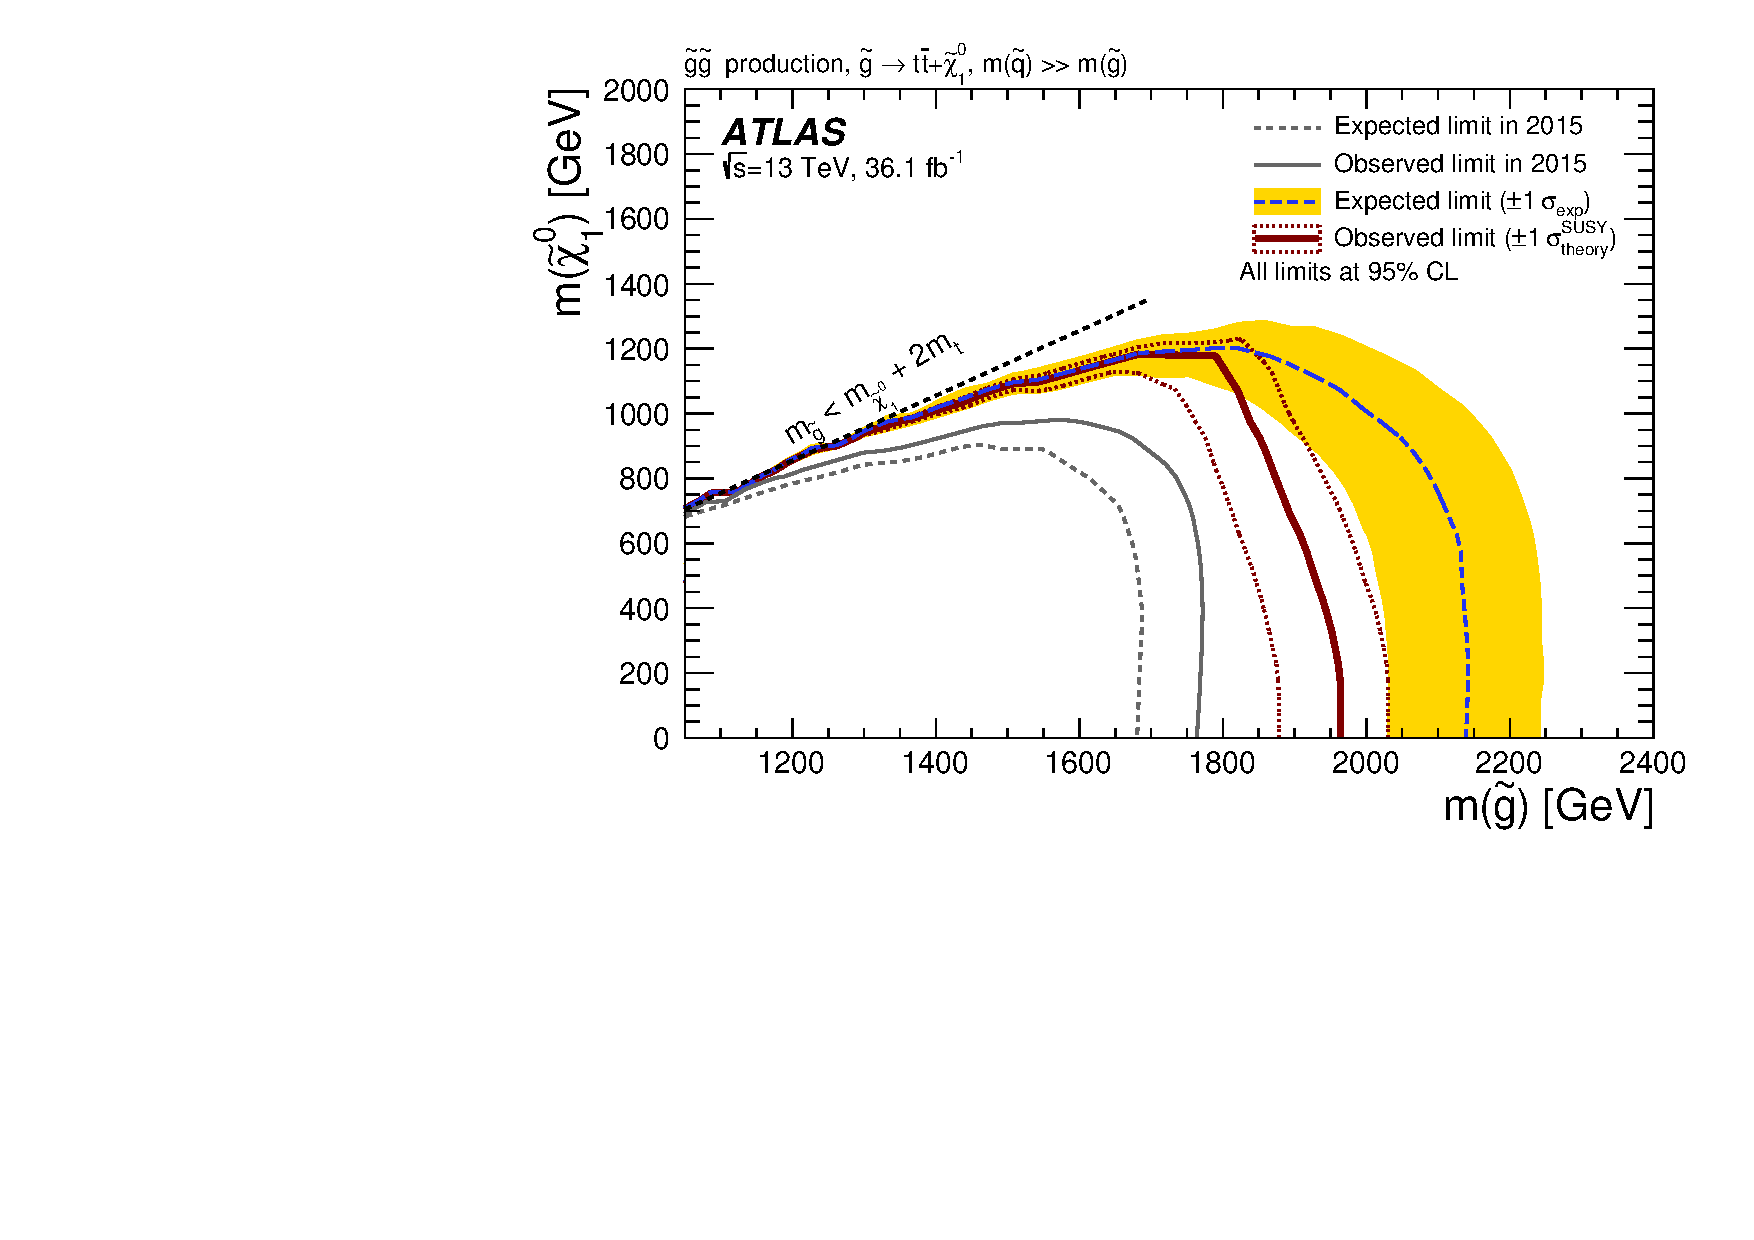
\includegraphics[width=0.75\textwidth]{figures/strong_prod/paper/limits/Limits_Gtt.pdf}\label{fig:limits_Gtt}}
	\subfigure[]{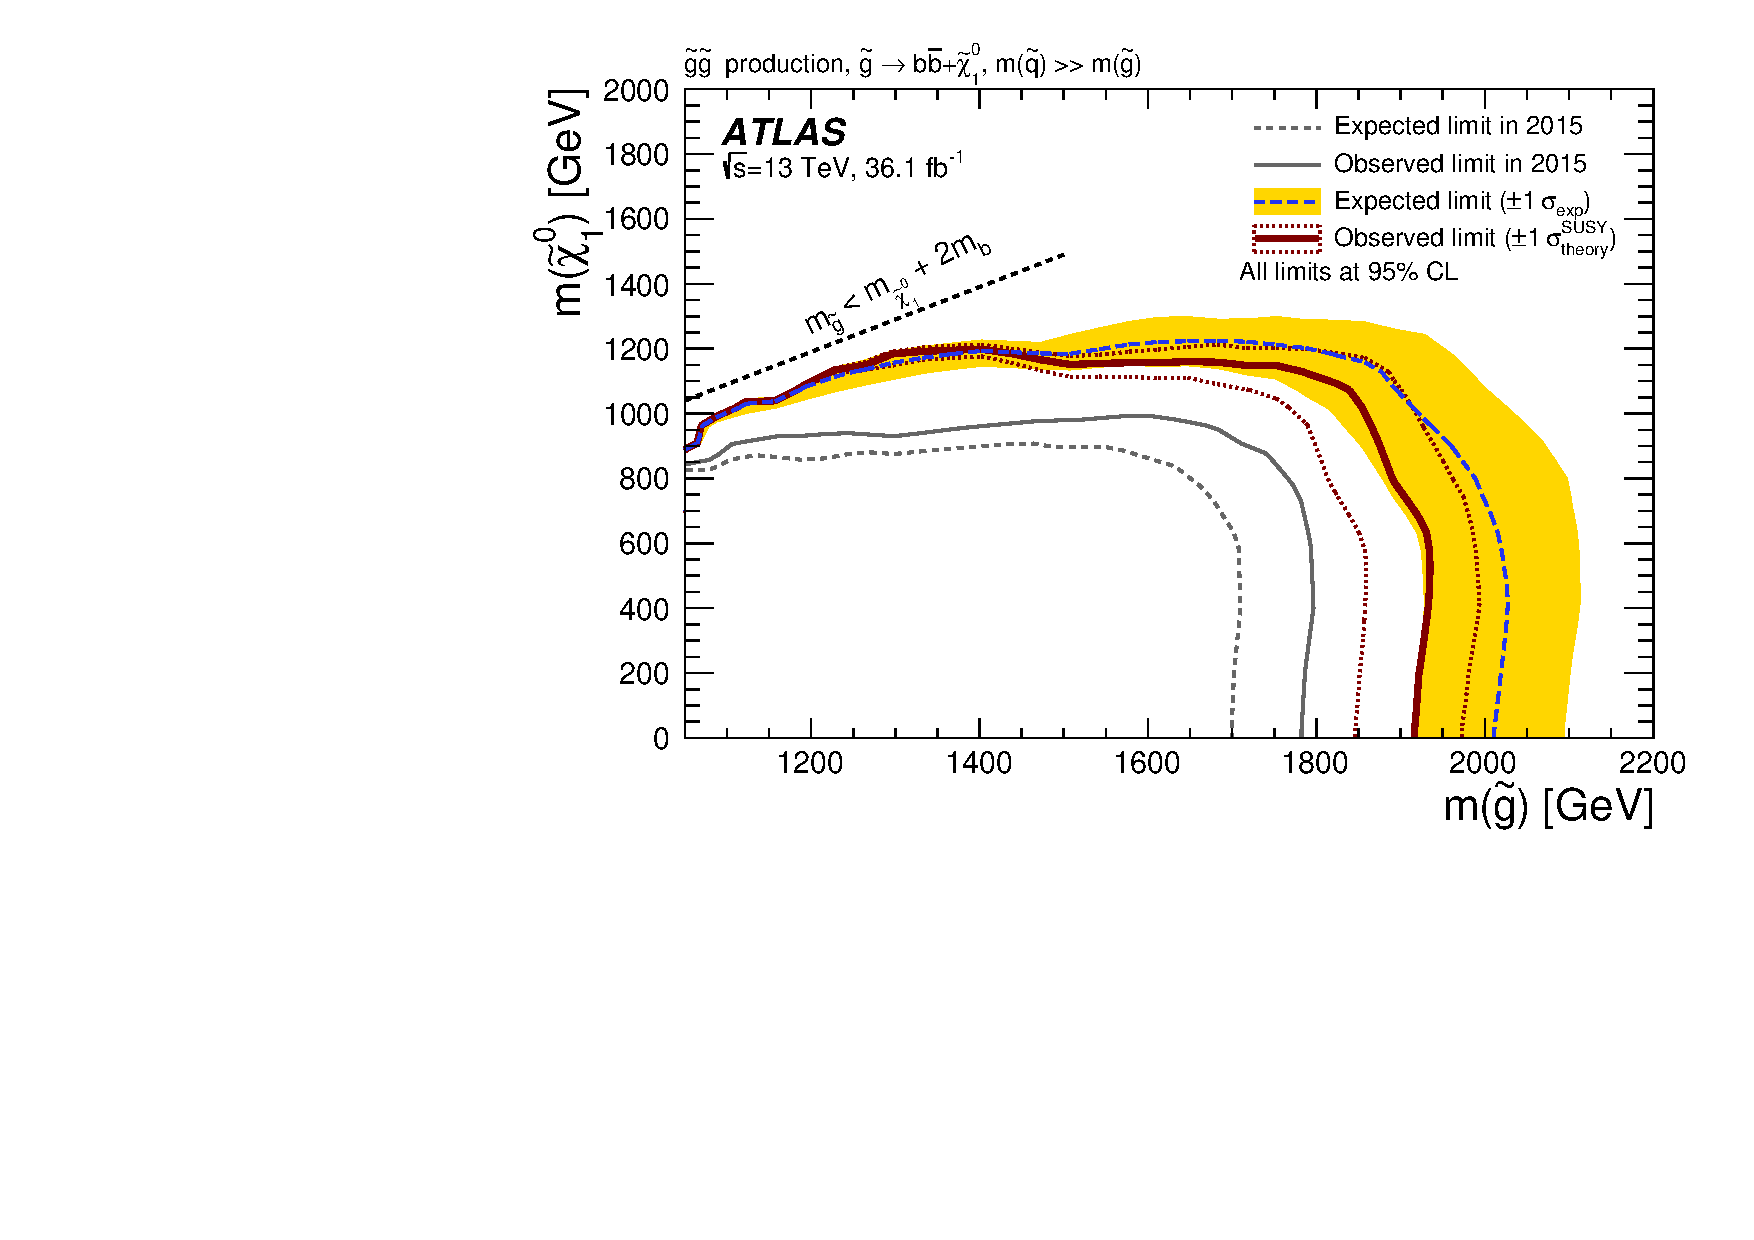
\includegraphics[width=0.75\textwidth]{figures/strong_prod/paper/limits/Limits_Gbb.pdf}\label{fig:limits_Gbb}}
	\caption{Exclusion limits in the $\ninoone$ and $\gluino$ mass plane
  		for the \subref{fig:limits_Gtt} Gtt and  \subref{fig:limits_Gbb} Gbb models obtained
		in the context of the multi-bin analysis. The dashed and solid bold lines
		show the 95\% CL expected and observed limits, respectively. The
  		shaded bands around the expected limits show the
                impact of the
  		experimental and background uncertainties. The dotted
  		lines show the impact on the observed limit of the variation of the
  		nominal signal cross-section by $\pm 1 \sigma$ of its theoretical
  		uncertainty. 
		The 95\%~CL expected and observed limits from the ATLAS search based on 2015 data 
  		\cite{Aad:2016eki} are also shown.  Figures from Ref. \cite{Aaboud:2017hrg}.}
	\label{fig:limits_GbbGtt}
\end{figure}

Figures \ref{fig:limits_Gtt} and \ref{fig:limits_Gbb} show the excluded region of the parameter space for Gtt and Gbb models 
respectively. The dashed blue lines show the expected 95\% \gls{cls} limit, which is the limit we would obtain if the observed number of 
events were identical to the expectation from \gls{sm} only, and the yellow bands around it indicate the effect of the 
uncertainty on the background predictions. The observed limits are shown with a solid red line, and the dotted red lines show the impact 
of the signal systematic uncertainties on the signal modeling (discussed in Section \ref{sec:strong:signalxsec}). 
Both in the case of the Gtt and Gbb models, the observed limit is weaker that the expected. 
This particularly evident for Gtt models with massless neutralino, where the limit is driven by SR-0L-HH, which has the larges deviation 
between expected and observed number of events.
The observed exclusion limit for massless neutralino is at around 1.97 and 1.92 for the Gtt and Gbb models respectively;
the sensitivity improves by 300 GeV and 450 GeV with respect to the Gbb and Gtt sensitivity obtained from the analysis of the 
2015 data \cite{Aad:2016eki}, shown with dashed black lines in Figure \ref{fig:limits_GbbGtt}. 
Note that the improvement in observed limits 
(comparing the solid black and the solid red lines) is much lower than that, since the analysis in Ref. \cite{Aad:2016eki}
observed a slight deficit while this analysis observes a slight excess. 

As discussed in Section \ref{sec:strong:signalmodel}, the results of the multi-bin analysis are also used to place 
limits on a more realistic model, where the gluino can decay to $ t \bar{t} \ninoone$, $ b \bar{b} \ninoone$, 
or $t \bar{b} \chinoonem$, and the $\chinoonem$ then decays to $\ninoone$ and soft fermions. All combinations of different \gls{br}
to these three decay modes with a unitary constraint on their sum are considered. 
The inclusion of the gluino \glspl{br} as additional parameters makes it impossible to show the results in the two-dimensional plane
defined by the masses of the gluino and the neutralino, as it is done for the simpler Gtt and Gbb models.
Instead, the limits are presented in the $B(\gluino \to t \bar{t} \ninoone)$-$B(\gluino \to b \bar{b} \ninoone)$ plane, 
assuming that $B(\gluino \to t \bar{b} \chinoonem) = 1 - B(\gluino \to t \bar{t} \ninoone) - B(\gluino \to b \bar{b} \ninoone)$, 
and only a few selected mass points are considered.  

Figure \ref{fig:limit_br_fixed_neu} shows the 95\% \gls{cls} exclusion limit for signal models with $m(\ninoone) = 1$ GeV and 
$m(\gluino) = 1.8$, 1.9 and 2.0 TeV. The solid and dashed lines show respectively the observed and expected limits for the different 
mass hypotheses, distinguished by the different colors. The hashing indicates which side of the plane is excluded. 
Due to the mild excesses observed in the multi-bin analysis, the observed limits are weaker than the expected. 
In particular, for a gluino mass of 1.8 TeV, we expect to exclude the entire \gls{br} plane, while the "pure Gtb" corner 
in the bottom left, where both $B(\gluino \to t \bar{t} \ninoone)$ and $B(\gluino \to b \bar{b} \ninoone)$ are low, 
is not excluded; none of the points are excluded for a gluino mass of 2.0 TeV. 

Figure \ref{fig:limit_br_fixed_glu} shows instead three signal mass hypotheses with a gluino mass of 1.9 TeV 
and $m(\ninoone) = 1$, 600 and 1000 GeV. Also in this case the observed limits are less stringent than the expected, leaving 
non-excluded areas also for signals that we expect to exclude for any \gls{br}, such as the one with neutralino mass of 600 GeV.


\begin{figure}[htbp]
	\centering
	\subfigure[]{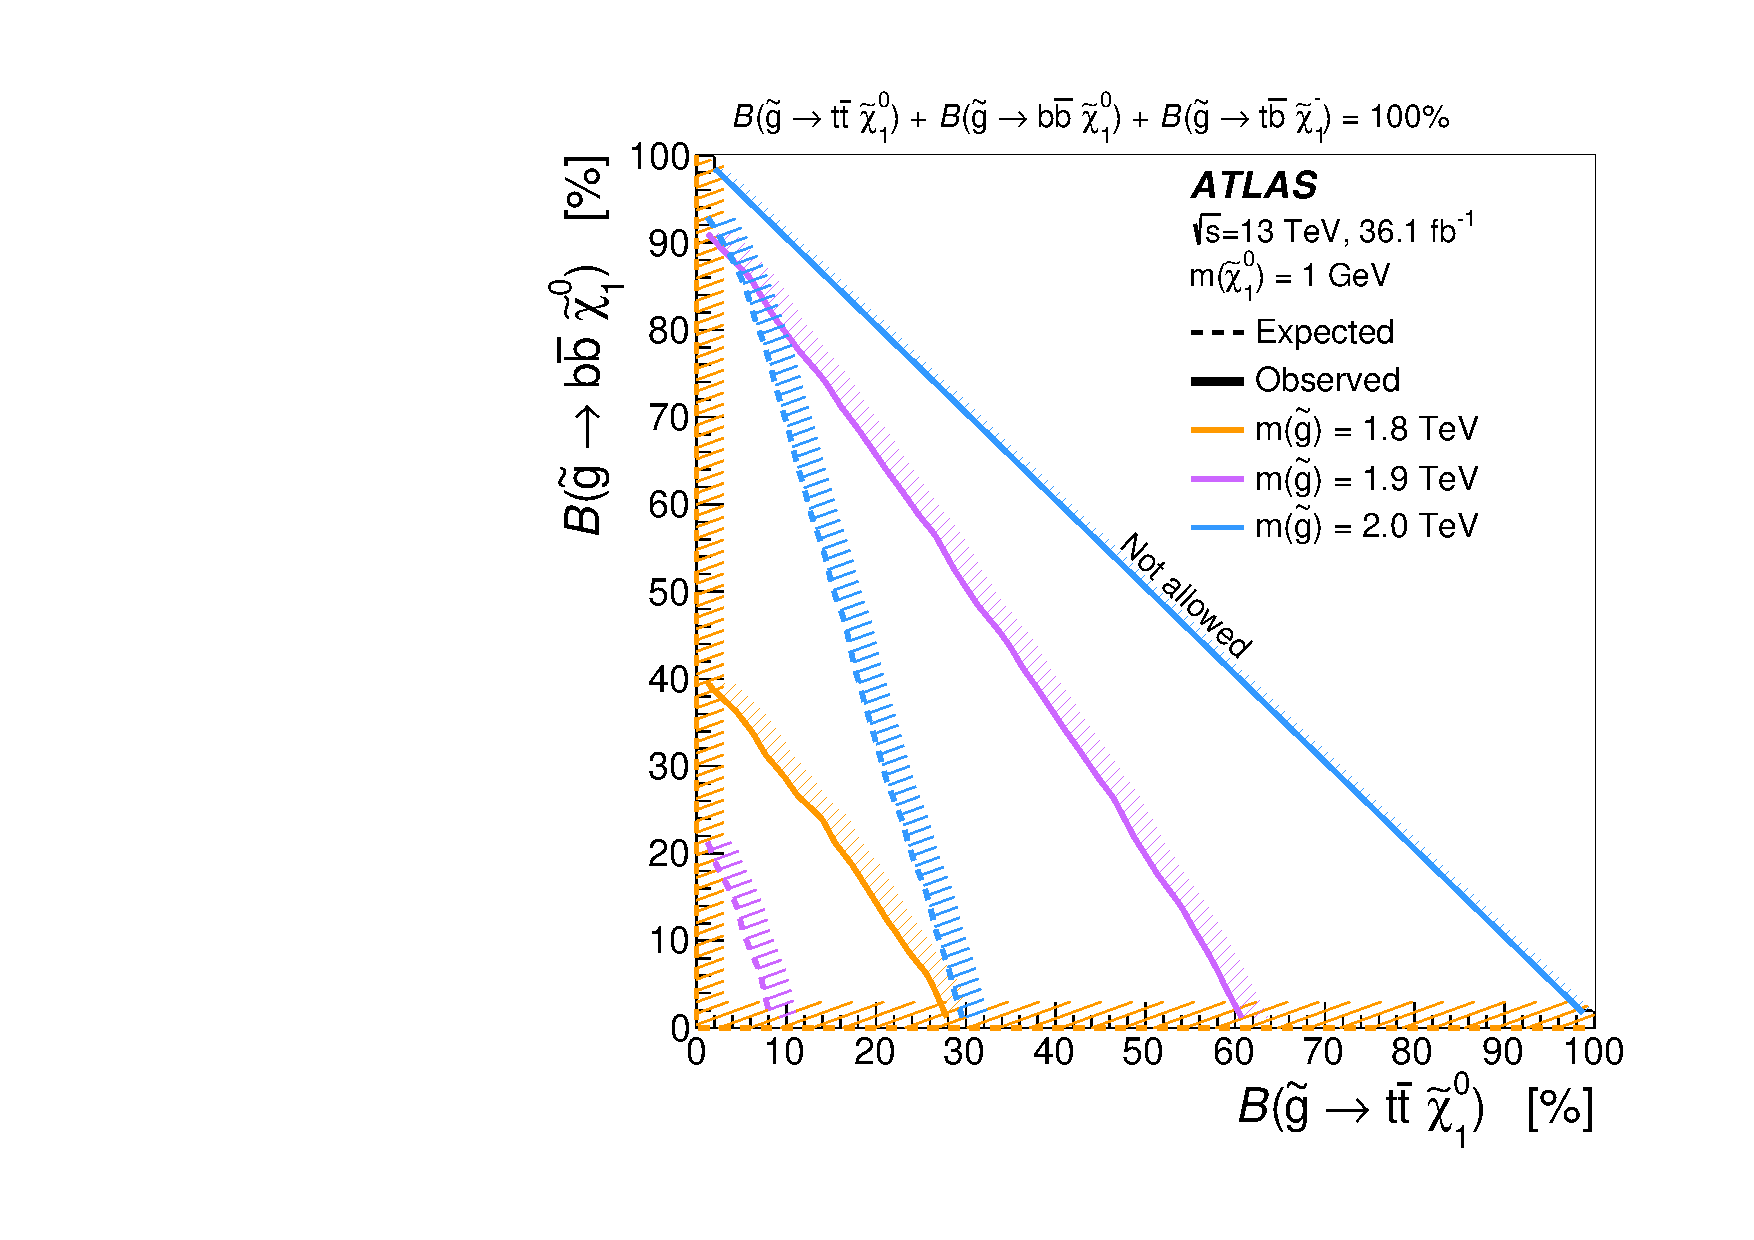
\includegraphics[width=0.63\textwidth]{figures/strong_prod/paper/limits/triangle_UL_massless_neutralino.pdf}\label{fig:limit_br_fixed_neu}}
	\subfigure[]{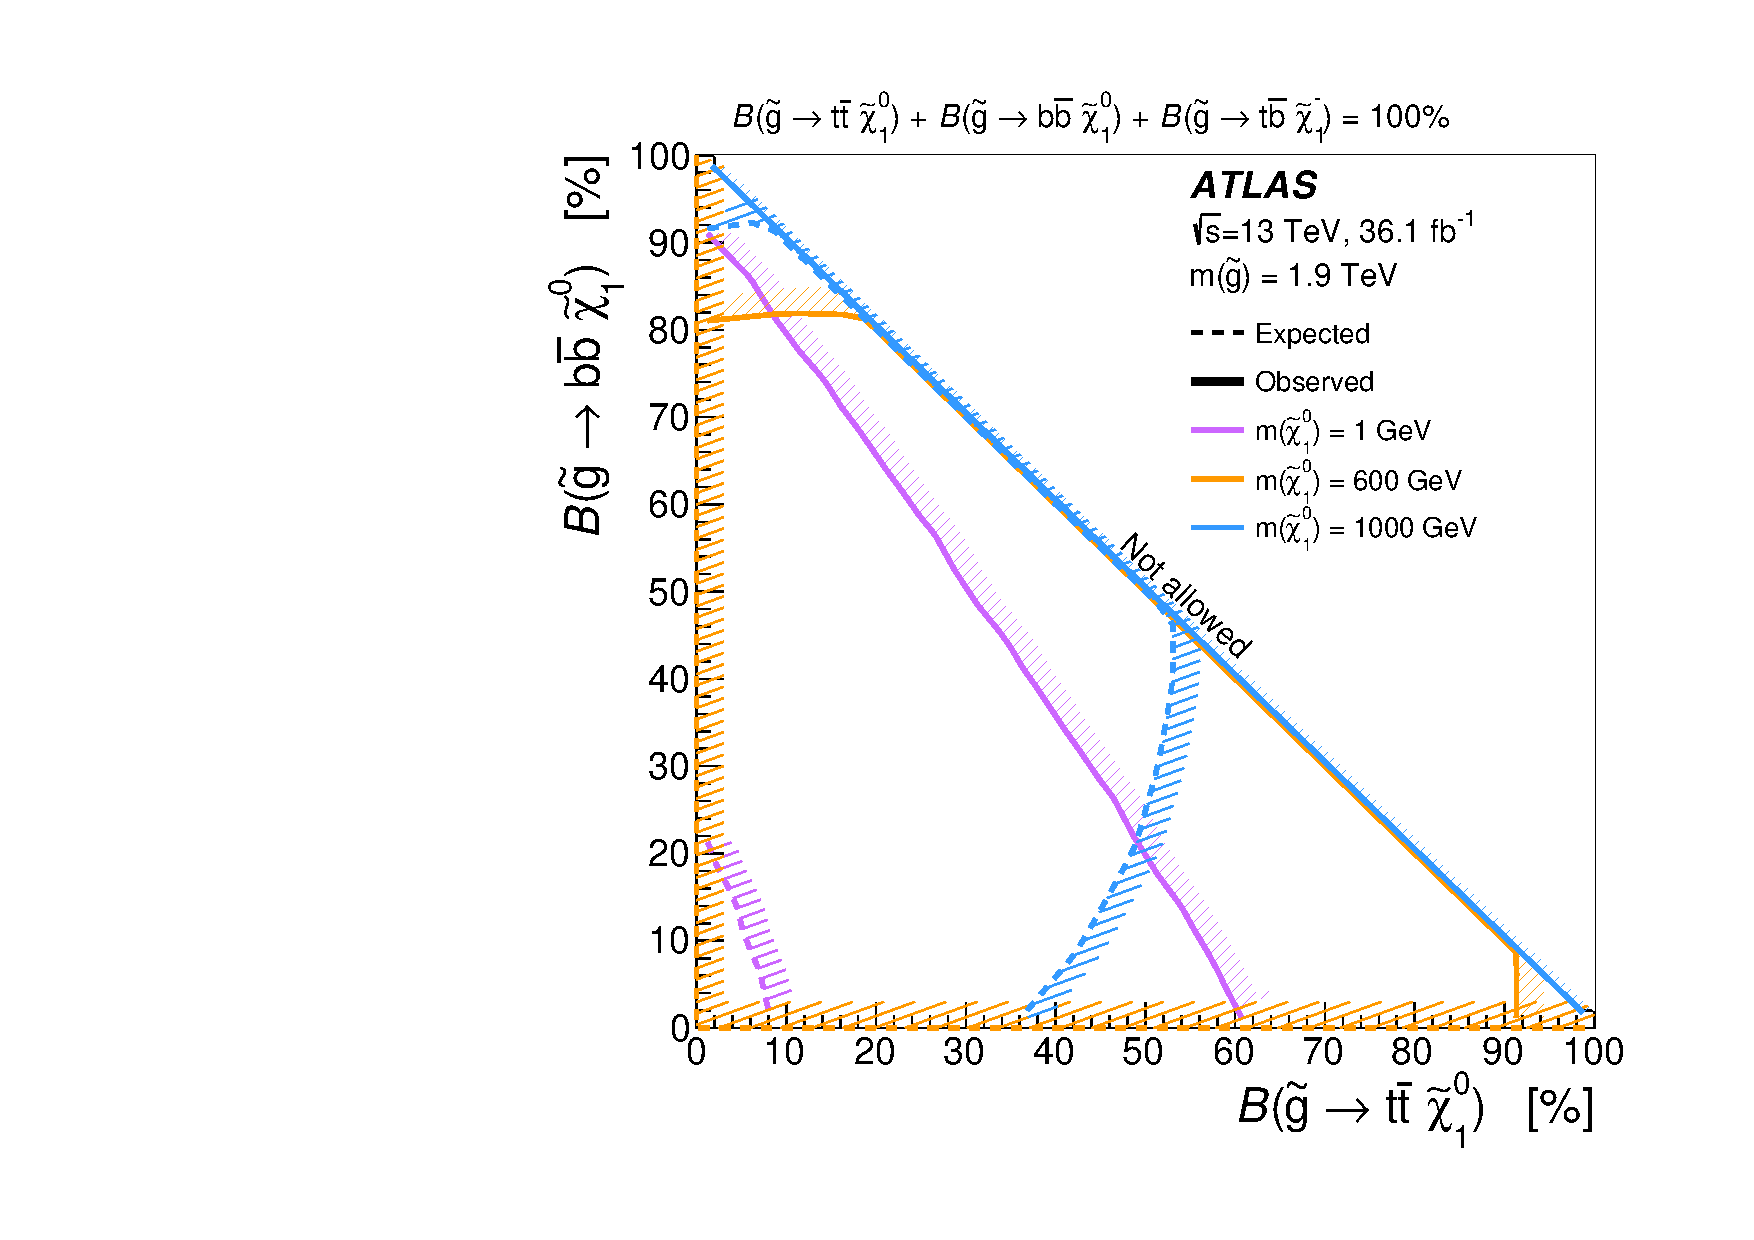
\includegraphics[width=0.63\textwidth]{figures/strong_prod/paper/limits/triangle_UL_1900_gluino.pdf}\label{fig:limit_br_fixed_glu}}
	\caption{Exclusion limits in the $\gluino \to t \bar{t} \ninoone$ and $\gluino \to b \bar{b} \ninoone$
		branching ratio plane assuming \subref{fig:limit_br_fixed_neu} a neutralino mass of 1 GeV and various gluino masses 
		(1.8, 1.9 and 2.0 TeV) and \subref{fig:limit_br_fixed_glu} a gluino mass of 1.9 TeV and three neutralino masses (1, 600 and 1000 GeV). 
		In \subref{fig:limit_br_fixed_neu}, the expected limit for a gluino mass of 1.8 TeV follows the plot axes, meaning that the whole plane is 
		expected to be excluded at 95\% CL.
		The dashed and solid bold lines show the 95\% CL expected and observed limits, respectively. The hashing indicates which side of the line 
		is excluded. The upper right half of the plane is forbidden by the requirement that the sum of branching ratios does not exceed 100\%.
		    Figures from Ref. \cite{Aaboud:2017hrg}.}
\end{figure}

\FloatBarrier

\section{Comparison of cut-and-count and multi-bin strategies}

In this analysis, the results of the multi-bin analysis are used to set model-dependent limits on selected signal models.
Also the regions cut-and-count analysis, used to set the model-independent limits in Section \ref{sec:strong:modelindepUL}, 
can be used to provide a statement on specific signal models. The different regions of the cut-and-count analysis are not orthogonal 
and therefore cannot be combined in a single statistical fit, but they can still be "visually combined" in a single exclusion contour 
by selecting for each mass point the cut-and-count region with the best expected sensitivity, and this contour can be compared 
with the contour obtained with the multi-bin approach.
This is shown in Figures \ref{fig:limits_Gtt_comp} and \ref{fig:limits_Gbb_comp} for the Gtt and Gbb models respectively.
Since we want to make a statement on the sensitivity of the two strategies, we compare only the expected exclusion contours 
(in blue for the cut-and-count analysis, in pink for the multi-bin analysis) and not the observed exclusion contours. 
The grey numbers on the figures represent the relative difference in expected upper limit on the signal strength: 
a negative number indicates a stronger limit from the multi-bin analysis. 
In the case of the Gtt grid in Figure \ref{fig:limits_Gtt_comp}, the multi-bin approach provides an improvement in 
expected upper limit of $\approx$30\% in the bulk of the mass plane, and up to $\approx$50\% for the more challenging 
kinematic regime where the mass of the neutralino is closer to the mass of the gluino.
In terms of gluino mass reach, this translates in an expected limit about 70 GeV stronger for massless neutralino.
In the case of the Gbb signal models, while it is still true that for most of the mass points the expected limit on the 
signal strength is better with the multi-bin approach, for the region of the parameter space with intermediate gluino and 
neutralino masses the cut-and-count analysis provides a stronger sensitivity.
This is balanced by a better sensitivity of the multi-bin strategy for $m(\gluino) \approx 2$ TeV, $m(\ninoone) \approx 700$
GeV (where the cut-and-count approach shows the negative impact of a switch in best-expected region for neighboring mass points),
and the two strategies have the same limit for massless neutralino. 
The reason of the different relative performance of multi-bin and cut-and-count approaches in the Gtt and Gbb signal 
models relies on the optimization strategy of the multi-bin analysis, which favors Gtt: the regions with intermediate 
number of jets, which could still be sensitive to Gbb models, are optimized based on Gtt signal benchmarks.



\begin{figure}[htbp]
	\centering 
	\subfigure[]{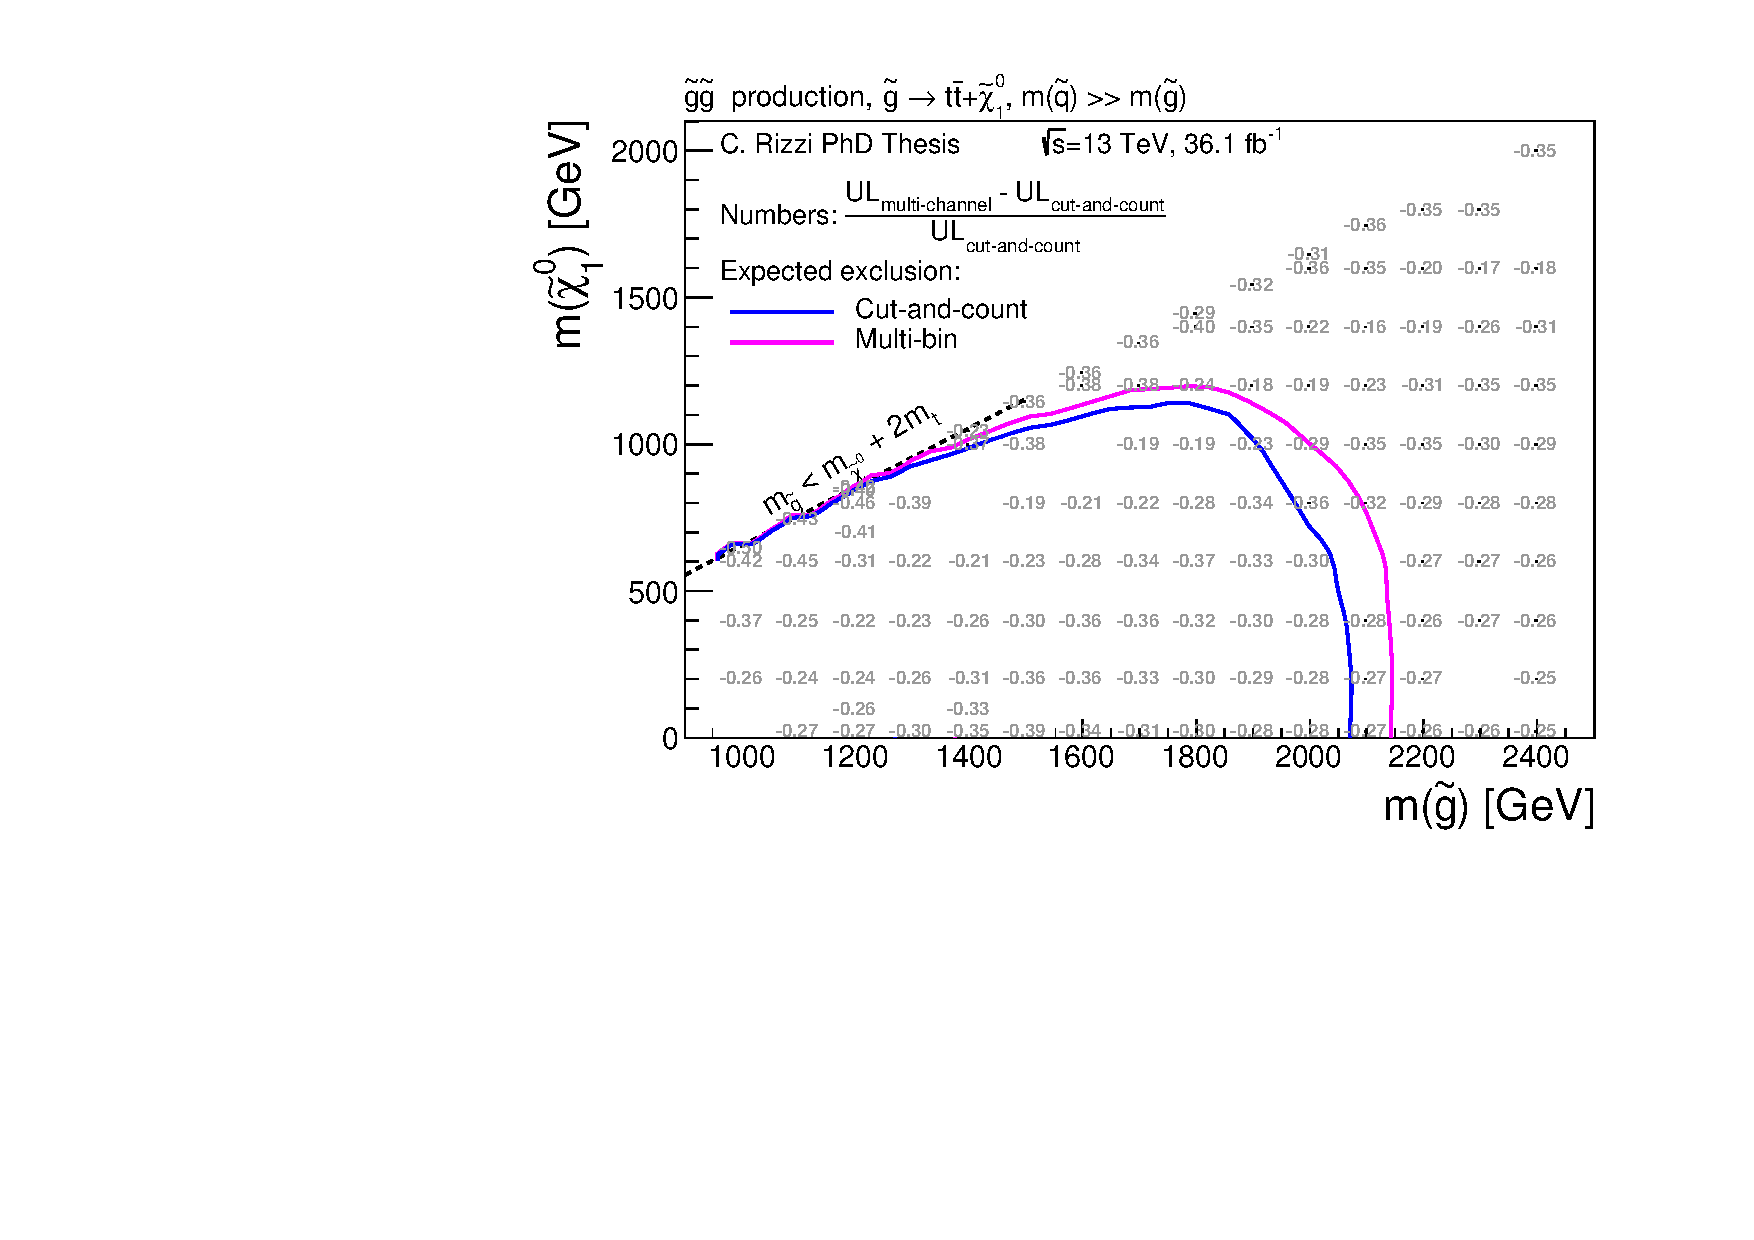
\includegraphics[width=0.75\textwidth]{figures/strong_prod/extra/UL_comp_combi_multich_Gtt.pdf}\label{fig:limits_Gtt_comp}}
	\subfigure[]{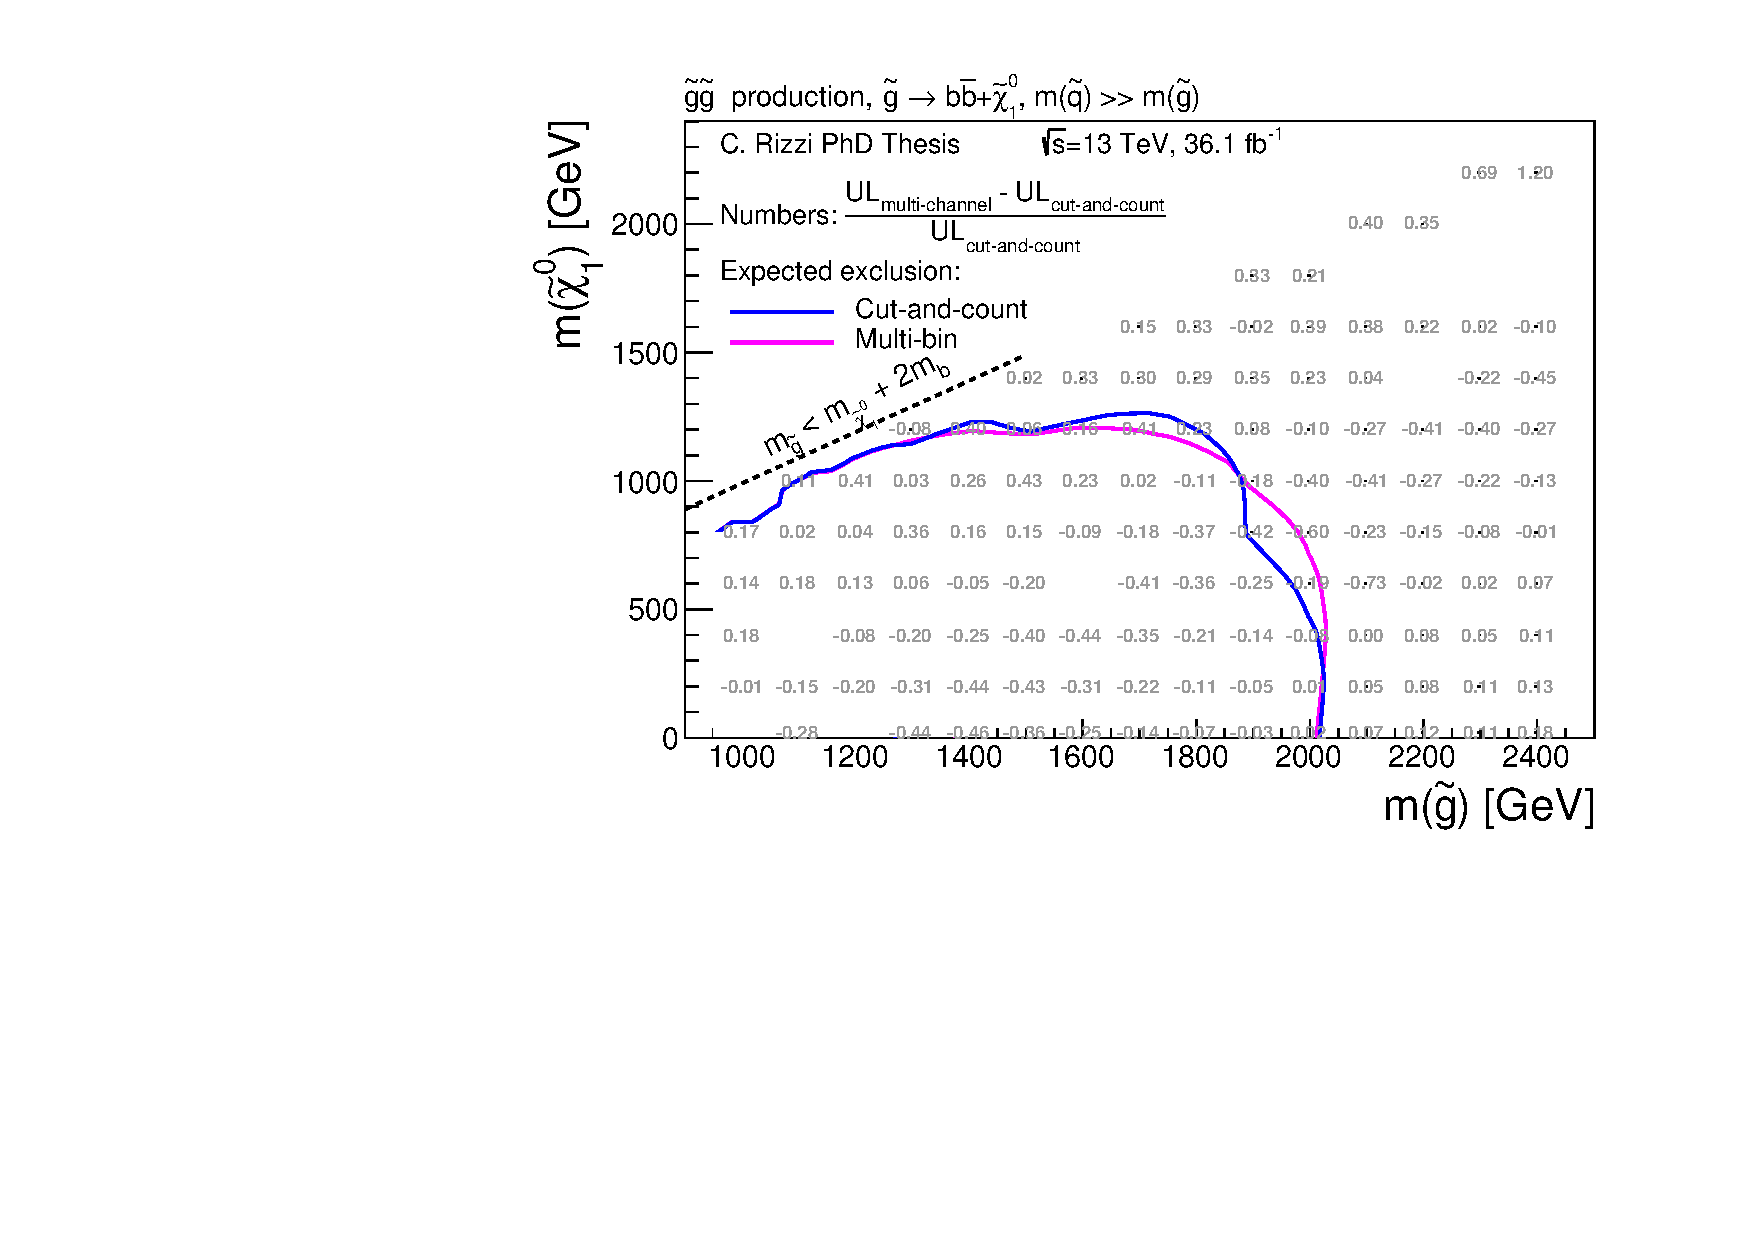
\includegraphics[width=0.75\textwidth]{figures/strong_prod/extra/UL_comp_combi_multich_Gbb.pdf}\label{fig:limits_Gbb_comp}}
	\caption{Exclusion limits in the $\ninoone$ and $\gluino$ mass plane
  		for the \subref{fig:limits_Gtt_comp} Gtt and  \subref{fig:limits_Gbb_comp} Gbb models obtained
		in the context of the multi-bin analysis (pink line) and of the cut-and-count analysis (blue line). 
		The gray numbers show the relative difference in expected \gls{ul} on the signal strength 
		between the multi-bin and the cut-and-count analysis: a negative number indicates a lower expected \gls{ul} for the multi-bin analysis. }
	\label{fig:limits_GbbGtt_comp}
\end{figure}

%\section{Results in the context of the ATLAS SUSY group}
